\subsection{The Stall}

\subsection{The Stall}

\subsection{The Stall}

\subsection{The Stall}

\input{plots/stall}

We will now explore stall-specific compression strategies.
Recall that the stall is the section of a read which occurs at
the beginning between the surge and pre-adapter surge. See Figure
\ref{fig:start-sections} for some context and Figure \ref{fig:stall} for a
close-up of the section. It is thought to occur due to the motor protein `stalling'
before it begins to unwind the molecule through the nanopore. It consists of
hundreds to thousands of data points which oscillate with little variation
around the read's median. The stall is a highly likely occurrence in any read,
for instance, only 6 reads in the data set do not have a stall.
However, its length varies from read to read, ranging from 34 to \num{37128}
with a mean of 1140.33. See Table \ref{tab:stall-n} for more information.

\input{plots/stall-n-tab}

Since this section oscillates with little variance around the read's median,
the maximum and minimum are much closer than in the DNA section.
Notably, the standard deviation of raw signal values in a stall is 5.72 compared
to 35.07 for the whole data set.
Instead of computing the zig-zag deltas we could transform the stall by subtract
its minimum point from all other stall points (FOR encoding) then
apply a suitable compression algorithm such as range coding. The idea is that
this could create a distribution with a lower entropy than the stall's zig-zag
deltas and hence more potential for compression.

Now we will define this strategy more formally. The \textit{stall} encoding
stores the stall's starting index (2 bytes), length (2 bytes), compressed size
(2 bytes) and compressed data (variable bytes) followed by the non-stall's
compressed size (4 bytes) and compressed data (variable bytes). The stall is
compressed using a \textit{stall-specific} encoding, whilst the non-stall is
compressed using a \textit{generic} algorithm.  See Figure \ref{fig:stall-enc}.
This method is more space-advantageous if
\[ C_{stall}(r) < C_{generic}(r) \]
where
\[ C_{stall}(r) = C_{specific}(r_s) + C_{generic}(r\setminus r_s) + 10. \]
In the above equations, $r\in\Omega$ is a read from the space of possible reads and $r_s$ is the
read's stall section. That is, this method is advantageous if its total
compressed size, consisting of the compressed stall, the compressed non-stall
and 10 bytes of metadata, is less than the usual encoding.

\input{plots/stall-enc}

The encoding could dynamically make the above comparison to decide
whether the stall is worth encoding or not. Then it could store an extra bit (or
byte for convenience) to flag whether the stall or generic algorithm is being
used. Let's name this algorithm the \textit{dynamic stall} encoding or
\textit{dstall} for short. See Figure \ref{fig:dstall-enc}. However, this extra
byte is a waste of space if the large majority of reads benefit from separate
stall encoding.

\input{plots/dstall-enc}

Consider our stall-specific encoding to be the FOR encoding followed by the
regular vbbe21 encoding (vbbe21) and range coding (altogether
\textit{rc-vbbe21-for}). Furthermore, let the generic algorithm be the
vbbe21-zd encoding followed by range coding (altogether
\textit{rc-vbbe21-zd}).
We shall name the stall encoding which uses the stall-specific encoding
rc-vbbe21-for and the generic encoding rc-vbbe21-zd: \textit{stall-fz}.
Similarly, we shall name \textit{dstall-fz} the dstall encoding which uses the
same stall-specific and generic encodings as stall-fz.

The compression ratio of stall-fz outperforms the generic method rc-vbbe21-zd
more often than not on reads with stalls of length greater than or equal to
1500. See Figure
\ref{fig:stall-best}. This means we could simply choose to encode the stall
separately when its length is at least 1500. Let's name this strategy
\textit{dstall-fz-1500}. Since most stalls are smaller than
1500 in size let's store an extra byte at the beginning of the encoding to flag
whether the stall is being encoded or not. If not, the stall specific section is
not recorded at all. This is equivalent to the dstall encoding in Figure
\ref{fig:dstall-enc} with the exception of how the stall encoding decision is
made. The advantage is that the read only needs to be compressed once rather
than twice as in the dstall algorithm. This is because dstall must compare
compressing the stall separately to not and so must check both ways before
proceeding. On the other hand, the dstall-fz-1500 strategy approximates the
dstall-fz decision boundary and hence should be faster during compression with
no speed difference during decompression. The compression ratio of
dstall-fz-1500 will not be better than dstall-fz but there should be little
difference if the decision boundary approximation is good.

%\input{plots/stall-ratio}
\input{plots/stall-best}


We will now explore stall-specific compression strategies.
Recall that the stall is the section of a read which occurs at
the beginning between the surge and pre-adapter surge. See Figure
\ref{fig:start-sections} for some context and Figure \ref{fig:stall} for a
close-up of the section. It is thought to occur due to the motor protein `stalling'
before it begins to unwind the molecule through the nanopore. It consists of
hundreds to thousands of data points which oscillate with little variation
around the read's median. The stall is a highly likely occurrence in any read,
for instance, only 6 reads in the data set do not have a stall.
However, its length varies from read to read, ranging from 34 to \num{37128}
with a mean of 1140.33. See Table \ref{tab:stall-n} for more information.

\begin{table}
    \caption{\label{tab:stall-n} Summary statistics of the data's stall lengths.}
    \begin{tabular}{|l|l|}
        \hline
Min & 34\\
	    Q1 & 314\\

Q2 & 771\\
	    Q3 & 1156\\
Max & 37128\\
\hline
Mean & 1140.33\\
	    Mode & 39\\
Sample SD & 1214.781\\
	\hline
    \end{tabular}
\end{table}


Since this section oscillates with little variance around the read's median,
the maximum and minimum are much closer than in the DNA section.
Notably, the standard deviation of raw signal values in a stall is 5.72 compared
to 35.07 for the whole data set.
Instead of computing the zig-zag deltas we could transform the stall by subtract
its minimum point from all other stall points (FOR encoding) then
apply a suitable compression algorithm such as range coding. The idea is that
this could create a distribution with a lower entropy than the stall's zig-zag
deltas and hence more potential for compression.

Now we will define this strategy more formally. The \textit{stall} encoding
stores the stall's starting index (2 bytes), length (2 bytes), compressed size
(2 bytes) and compressed data (variable bytes) followed by the non-stall's
compressed size (4 bytes) and compressed data (variable bytes). The stall is
compressed using a \textit{stall-specific} encoding, whilst the non-stall is
compressed using a \textit{generic} algorithm.  See Figure \ref{fig:stall-enc}.
This method is more space-advantageous if
\[ C_{stall}(r) < C_{generic}(r) \]
where
\[ C_{stall}(r) = C_{specific}(r_s) + C_{generic}(r\setminus r_s) + 10. \]
In the above equations, $r\in\Omega$ is a read from the space of possible reads and $r_s$ is the
read's stall section. That is, this method is advantageous if its total
compressed size, consisting of the compressed stall, the compressed non-stall
and 10 bytes of metadata, is less than the usual encoding.

\begin{figure}
\centering\begin{tikzpicture}[node distance=0cm,start chain=1 going right,start chain=2 going right] \footnotesize
  \tikzstyle{mytape}=[draw,minimum height=1.5cm]
	\node(A1)  [on chain=1,mytape,fill=yellow!20] {$\underbrace{\overbracket{\text{ }p\text{ }}^{\text{2 bytes}}}_{\text{stall start position}}$};
	\node(A2)  [on chain=1,mytape,fill=yellow!20] {$\underbrace{\overbracket{|r_s|}^{\text{2 bytes}}}_{\text{stall length}}$};
	\node(A3)  [on chain=1,mytape,fill=yellow!20] {$\underbrace{\overbracket{m_s}^{\text{2 bytes}}}_{\text{stall compressed size}}$};
	\node(A4)  [on chain=1,mytape,fill=green!20] {$\underbrace{\overbracket{C_{specific}(r_s)}^{m_s\text{ bytes}}}_{\text{stall compressed data}}$};
	\node(B1)  [on chain=1,mytape,fill=yellow!35] {$\underbrace{\overbracket{m}^{\text{4 bytes}}}_{\text{non-stall compressed size}}$};
	\node(B2)  [on chain=1,mytape,fill=green!35] {$\underbrace{\overbracket{C_{generic}(r\setminus r_s)}^{m\text{ bytes}}}_{\text{non-stall compressed data}}$};
\end{tikzpicture}
	\caption{\label{fig:stall-enc}The stall encoding records the stall's
starting position in the read, length, compressed size and compressed data,
	followed by the non-stall's compressed size and compressed data.
	The specific and generic compression algorithms used are known
	beforehand and hence are not stored. stall-fz uses rccm-vbbe21-for and
	rccm-vbbe21-zd as the specific and generic algorithm respectively.}
\end{figure}


The encoding could dynamically make the above comparison to decide
whether the stall is worth encoding or not. Then it could store an extra bit (or
byte for convenience) to flag whether the stall or generic algorithm is being
used. Let's name this algorithm the \textit{dynamic stall} encoding or
\textit{dstall} for short. See Figure \ref{fig:dstall-enc}. However, this extra
byte is a waste of space if the large majority of reads benefit from separate
stall encoding.

\usetikzlibrary{decorations.pathreplacing,positioning,calc}

\begin{figure}
\centering\begin{tikzpicture}[node distance=0cm,start chain=1 going right,start chain=2 going right] \footnotesize
  \tikzstyle{mytape}=[draw,minimum height=1.5cm]
	\node(A0)  [on chain=1,mytape,fill=blue!20] {$\underbrace{\overbracket{flag}^{\text{1 byte}}}_{\text{stall encoded flag}}$};
	\node(A1)  [on chain=1,mytape,fill=yellow!20] {$\underbrace{\overbracket{\text{ }p\text{ }}^{\text{2 bytes}}}_{\text{stall start position}}$};
	\node(A2)  [on chain=1,mytape,fill=yellow!20] {$\underbrace{\overbracket{|r_s|}^{\text{2 bytes}}}_{\text{stall length}}$};
	\node(A3)  [on chain=1,mytape,fill=yellow!20] {$\underbrace{\overbracket{m_s}^{\text{2 bytes}}}_{\text{stall compressed size}}$};
	\node(A4)  [on chain=1,mytape,fill=green!20] {$\underbrace{\overbracket{C_{specific}(r_s)}^{m_s\text{ bytes}}}_{\text{stall compressed data}}$};
	\node(B1)  [on chain=1,mytape,fill=yellow!35] {$\underbrace{\overbracket{m}^{\text{4 bytes}}}_{\text{non-stall compressed size}}$};
	\node(B2)  [on chain=1,mytape,fill=green!35] {$\underbrace{\overbracket{C_{generic}(r\setminus r_s)}^{m\text{ bytes}}}_{\text{non-stall compressed data}}$};
	\draw
	[decorate,decoration={brace,amplitude=5pt,mirror,raise=4ex}]
	  ($(A1)-(0,0.3)$) -- ($(A4)-(0,0.3)$) node[midway,yshift=-3em]{if $flag=1$};
\end{tikzpicture}
	\caption{\label{fig:dstall-enc}The dstall encoding stores an extra byte
	at the beginning to mark whether the stall is being encoded or not. If
	it is being encoded the remaining data matches the stall encoding.
	Otherwise, $r_s$ is empty and the whole read is compressed using the
	generic algorithm as usual. That is, the read's compressed size (4
	bytes) and data follows the flag.}
\end{figure}


Consider our stall-specific encoding to be the FOR encoding followed by the
regular vbbe21 encoding (vbbe21) and range coding (altogether
\textit{rc-vbbe21-for}). Furthermore, let the generic algorithm be the
vbbe21-zd encoding followed by range coding (altogether
\textit{rc-vbbe21-zd}).
We shall name the stall encoding which uses the stall-specific encoding
rc-vbbe21-for and the generic encoding rc-vbbe21-zd: \textit{stall-fz}.
Similarly, we shall name \textit{dstall-fz} the dstall encoding which uses the
same stall-specific and generic encodings as stall-fz.

The compression ratio of stall-fz outperforms the generic method rc-vbbe21-zd
more often than not on reads with stalls of length greater than or equal to
1500. See Figure
\ref{fig:stall-best}. This means we could simply choose to encode the stall
separately when its length is at least 1500. Let's name this strategy
\textit{dstall-fz-1500}. Since most stalls are smaller than
1500 in size let's store an extra byte at the beginning of the encoding to flag
whether the stall is being encoded or not. If not, the stall specific section is
not recorded at all. This is equivalent to the dstall encoding in Figure
\ref{fig:dstall-enc} with the exception of how the stall encoding decision is
made. The advantage is that the read only needs to be compressed once rather
than twice as in the dstall algorithm. This is because dstall must compare
compressing the stall separately to not and so must check both ways before
proceeding. On the other hand, the dstall-fz-1500 strategy approximates the
dstall-fz decision boundary and hence should be faster during compression with
no speed difference during decompression. The compression ratio of
dstall-fz-1500 will not be better than dstall-fz but there should be little
difference if the decision boundary approximation is good.

%\begin{figure}
\centering
\input{plots/reads.blow5.test.svbbe21.read.prop}
\caption{\label{fig:stall-ratio}The 100\% stacked histogram of the compression
	methods with the highest compression ratio for all the reads in the data
	versus their stall length. Reads with a stall length $\sim$1500 and
	greater are more likely to be compressed smaller using stall-fz than
	rc-vbbe21-zd.}
\end{figure}

\begin{figure}
\centering
%\input{plots/reads.blow5.test.svbbe21.read.best}
\includegraphics[scale=0.7]{plots/reads.blow5.test.svbbe21.read.update.best.pdf}
	\caption[A scatter plot of the compression methods with
the highest compression ratio on each read out of rc01s-vbbe21-zd and stall-fz.]{\label{fig:stall-best}A scatter plot of the compression methods with
the highest compression ratio on each read out of rc01s-vbbe21-zd and stall-fz. The
best compression ratio is plotted against the length of the read's stall. Reads
with a stall length $\sim$1500 and greater are more likely to be compressed
smaller with stall-fz rather than rc01s-vbbe21-zd.}
\end{figure}



We will now explore stall-specific compression strategies.
Recall that the stall is the section of a read which occurs at
the beginning between the surge and pre-adapter surge. See Figure
\ref{fig:start-sections} for some context and Figure \ref{fig:stall} for a
close-up of the section. It is thought to occur due to the motor protein `stalling'
before it begins to unwind the molecule through the nanopore. It consists of
hundreds to thousands of data points which oscillate with little variation
around the read's median. The stall is a highly likely occurrence in any read,
for instance, only 6 reads in the data set do not have a stall.
However, its length varies from read to read, ranging from 34 to \num{37128}
with a mean of 1140.33. See Table \ref{tab:stall-n} for more information.

\begin{table}
    \caption{\label{tab:stall-n} Summary statistics of the data's stall lengths.}
    \begin{tabular}{|l|l|}
        \hline
Min & 34\\
	    Q1 & 314\\

Q2 & 771\\
	    Q3 & 1156\\
Max & 37128\\
\hline
Mean & 1140.33\\
	    Mode & 39\\
Sample SD & 1214.781\\
	\hline
    \end{tabular}
\end{table}


Since this section oscillates with little variance around the read's median,
the maximum and minimum are much closer than in the DNA section.
Notably, the standard deviation of raw signal values in a stall is 5.72 compared
to 35.07 for the whole data set.
Instead of computing the zig-zag deltas we could transform the stall by subtract
its minimum point from all other stall points (FOR encoding) then
apply a suitable compression algorithm such as range coding. The idea is that
this could create a distribution with a lower entropy than the stall's zig-zag
deltas and hence more potential for compression.

Now we will define this strategy more formally. The \textit{stall} encoding
stores the stall's starting index (2 bytes), length (2 bytes), compressed size
(2 bytes) and compressed data (variable bytes) followed by the non-stall's
compressed size (4 bytes) and compressed data (variable bytes). The stall is
compressed using a \textit{stall-specific} encoding, whilst the non-stall is
compressed using a \textit{generic} algorithm.  See Figure \ref{fig:stall-enc}.
This method is more space-advantageous if
\[ C_{stall}(r) < C_{generic}(r) \]
where
\[ C_{stall}(r) = C_{specific}(r_s) + C_{generic}(r\setminus r_s) + 10. \]
In the above equations, $r\in\Omega$ is a read from the space of possible reads and $r_s$ is the
read's stall section. That is, this method is advantageous if its total
compressed size, consisting of the compressed stall, the compressed non-stall
and 10 bytes of metadata, is less than the usual encoding.

\begin{figure}
\centering\begin{tikzpicture}[node distance=0cm,start chain=1 going right,start chain=2 going right] \footnotesize
  \tikzstyle{mytape}=[draw,minimum height=1.5cm]
	\node(A1)  [on chain=1,mytape,fill=yellow!20] {$\underbrace{\overbracket{\text{ }p\text{ }}^{\text{2 bytes}}}_{\text{stall start position}}$};
	\node(A2)  [on chain=1,mytape,fill=yellow!20] {$\underbrace{\overbracket{|r_s|}^{\text{2 bytes}}}_{\text{stall length}}$};
	\node(A3)  [on chain=1,mytape,fill=yellow!20] {$\underbrace{\overbracket{m_s}^{\text{2 bytes}}}_{\text{stall compressed size}}$};
	\node(A4)  [on chain=1,mytape,fill=green!20] {$\underbrace{\overbracket{C_{specific}(r_s)}^{m_s\text{ bytes}}}_{\text{stall compressed data}}$};
	\node(B1)  [on chain=1,mytape,fill=yellow!35] {$\underbrace{\overbracket{m}^{\text{4 bytes}}}_{\text{non-stall compressed size}}$};
	\node(B2)  [on chain=1,mytape,fill=green!35] {$\underbrace{\overbracket{C_{generic}(r\setminus r_s)}^{m\text{ bytes}}}_{\text{non-stall compressed data}}$};
\end{tikzpicture}
	\caption{\label{fig:stall-enc}The stall encoding records the stall's
starting position in the read, length, compressed size and compressed data,
	followed by the non-stall's compressed size and compressed data.
	The specific and generic compression algorithms used are known
	beforehand and hence are not stored. stall-fz uses rccm-vbbe21-for and
	rccm-vbbe21-zd as the specific and generic algorithm respectively.}
\end{figure}


The encoding could dynamically make the above comparison to decide
whether the stall is worth encoding or not. Then it could store an extra bit (or
byte for convenience) to flag whether the stall or generic algorithm is being
used. Let's name this algorithm the \textit{dynamic stall} encoding or
\textit{dstall} for short. See Figure \ref{fig:dstall-enc}. However, this extra
byte is a waste of space if the large majority of reads benefit from separate
stall encoding.

\usetikzlibrary{decorations.pathreplacing,positioning,calc}

\begin{figure}
\centering\begin{tikzpicture}[node distance=0cm,start chain=1 going right,start chain=2 going right] \footnotesize
  \tikzstyle{mytape}=[draw,minimum height=1.5cm]
	\node(A0)  [on chain=1,mytape,fill=blue!20] {$\underbrace{\overbracket{flag}^{\text{1 byte}}}_{\text{stall encoded flag}}$};
	\node(A1)  [on chain=1,mytape,fill=yellow!20] {$\underbrace{\overbracket{\text{ }p\text{ }}^{\text{2 bytes}}}_{\text{stall start position}}$};
	\node(A2)  [on chain=1,mytape,fill=yellow!20] {$\underbrace{\overbracket{|r_s|}^{\text{2 bytes}}}_{\text{stall length}}$};
	\node(A3)  [on chain=1,mytape,fill=yellow!20] {$\underbrace{\overbracket{m_s}^{\text{2 bytes}}}_{\text{stall compressed size}}$};
	\node(A4)  [on chain=1,mytape,fill=green!20] {$\underbrace{\overbracket{C_{specific}(r_s)}^{m_s\text{ bytes}}}_{\text{stall compressed data}}$};
	\node(B1)  [on chain=1,mytape,fill=yellow!35] {$\underbrace{\overbracket{m}^{\text{4 bytes}}}_{\text{non-stall compressed size}}$};
	\node(B2)  [on chain=1,mytape,fill=green!35] {$\underbrace{\overbracket{C_{generic}(r\setminus r_s)}^{m\text{ bytes}}}_{\text{non-stall compressed data}}$};
	\draw
	[decorate,decoration={brace,amplitude=5pt,mirror,raise=4ex}]
	  ($(A1)-(0,0.3)$) -- ($(A4)-(0,0.3)$) node[midway,yshift=-3em]{if $flag=1$};
\end{tikzpicture}
	\caption{\label{fig:dstall-enc}The dstall encoding stores an extra byte
	at the beginning to mark whether the stall is being encoded or not. If
	it is being encoded the remaining data matches the stall encoding.
	Otherwise, $r_s$ is empty and the whole read is compressed using the
	generic algorithm as usual. That is, the read's compressed size (4
	bytes) and data follows the flag.}
\end{figure}


Consider our stall-specific encoding to be the FOR encoding followed by the
regular vbbe21 encoding (vbbe21) and range coding (altogether
\textit{rc-vbbe21-for}). Furthermore, let the generic algorithm be the
vbbe21-zd encoding followed by range coding (altogether
\textit{rc-vbbe21-zd}).
We shall name the stall encoding which uses the stall-specific encoding
rc-vbbe21-for and the generic encoding rc-vbbe21-zd: \textit{stall-fz}.
Similarly, we shall name \textit{dstall-fz} the dstall encoding which uses the
same stall-specific and generic encodings as stall-fz.

The compression ratio of stall-fz outperforms the generic method rc-vbbe21-zd
more often than not on reads with stalls of length greater than or equal to
1500. See Figure
\ref{fig:stall-best}. This means we could simply choose to encode the stall
separately when its length is at least 1500. Let's name this strategy
\textit{dstall-fz-1500}. Since most stalls are smaller than
1500 in size let's store an extra byte at the beginning of the encoding to flag
whether the stall is being encoded or not. If not, the stall specific section is
not recorded at all. This is equivalent to the dstall encoding in Figure
\ref{fig:dstall-enc} with the exception of how the stall encoding decision is
made. The advantage is that the read only needs to be compressed once rather
than twice as in the dstall algorithm. This is because dstall must compare
compressing the stall separately to not and so must check both ways before
proceeding. On the other hand, the dstall-fz-1500 strategy approximates the
dstall-fz decision boundary and hence should be faster during compression with
no speed difference during decompression. The compression ratio of
dstall-fz-1500 will not be better than dstall-fz but there should be little
difference if the decision boundary approximation is good.

%\begin{figure}
\centering
% Created by tikzDevice version 0.12.3.1 on 2022-10-21 15:39:01
% !TEX encoding = UTF-8 Unicode
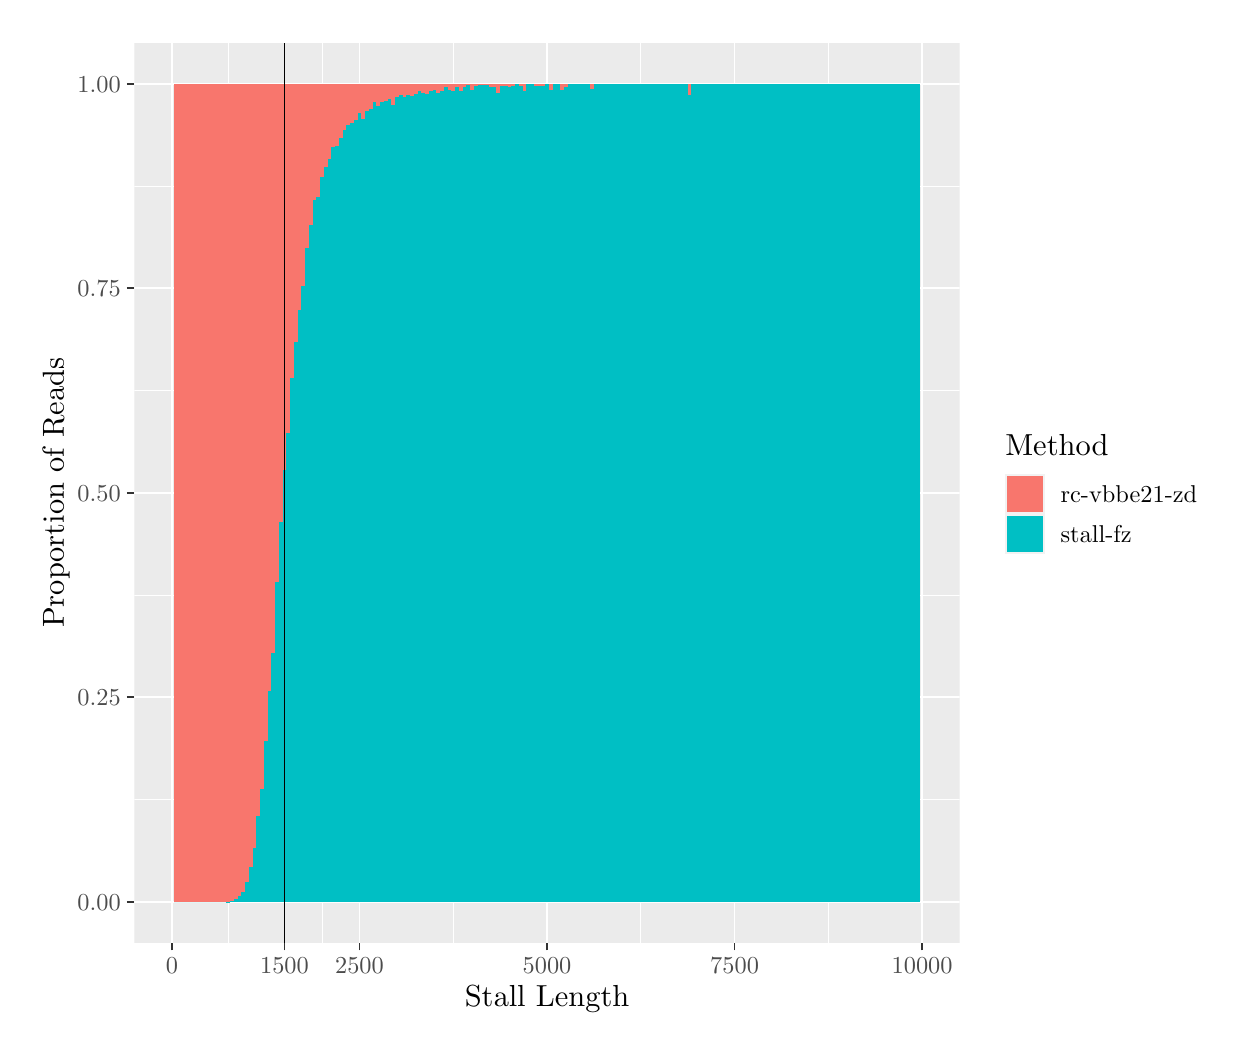
\begin{tikzpicture}[x=1pt,y=1pt]
\definecolor{fillColor}{RGB}{255,255,255}
\path[use as bounding box,fill=fillColor,fill opacity=0.00] (0,0) rectangle (433.62,361.35);
\begin{scope}
\path[clip] (  0.00,  0.00) rectangle (433.62,361.35);
\definecolor{drawColor}{RGB}{255,255,255}
\definecolor{fillColor}{RGB}{255,255,255}

\path[draw=drawColor,line width= 0.6pt,line join=round,line cap=round,fill=fillColor] (  0.00,  0.00) rectangle (433.62,361.35);
\end{scope}
\begin{scope}
\path[clip] ( 38.56, 30.69) rectangle (336.78,355.85);
\definecolor{fillColor}{gray}{0.92}

\path[fill=fillColor] ( 38.56, 30.69) rectangle (336.78,355.85);
\definecolor{drawColor}{RGB}{255,255,255}

\path[draw=drawColor,line width= 0.3pt,line join=round] ( 38.56, 82.42) --
	(336.78, 82.42);

\path[draw=drawColor,line width= 0.3pt,line join=round] ( 38.56,156.32) --
	(336.78,156.32);

\path[draw=drawColor,line width= 0.3pt,line join=round] ( 38.56,230.22) --
	(336.78,230.22);

\path[draw=drawColor,line width= 0.3pt,line join=round] ( 38.56,304.12) --
	(336.78,304.12);

\path[draw=drawColor,line width= 0.3pt,line join=round] ( 72.44, 30.69) --
	( 72.44,355.85);

\path[draw=drawColor,line width= 0.3pt,line join=round] (106.33, 30.69) --
	(106.33,355.85);

\path[draw=drawColor,line width= 0.3pt,line join=round] (153.78, 30.69) --
	(153.78,355.85);

\path[draw=drawColor,line width= 0.3pt,line join=round] (221.55, 30.69) --
	(221.55,355.85);

\path[draw=drawColor,line width= 0.3pt,line join=round] (289.33, 30.69) --
	(289.33,355.85);

\path[draw=drawColor,line width= 0.6pt,line join=round] ( 38.56, 45.47) --
	(336.78, 45.47);

\path[draw=drawColor,line width= 0.6pt,line join=round] ( 38.56,119.37) --
	(336.78,119.37);

\path[draw=drawColor,line width= 0.6pt,line join=round] ( 38.56,193.27) --
	(336.78,193.27);

\path[draw=drawColor,line width= 0.6pt,line join=round] ( 38.56,267.17) --
	(336.78,267.17);

\path[draw=drawColor,line width= 0.6pt,line join=round] ( 38.56,341.07) --
	(336.78,341.07);

\path[draw=drawColor,line width= 0.6pt,line join=round] ( 52.11, 30.69) --
	( 52.11,355.85);

\path[draw=drawColor,line width= 0.6pt,line join=round] ( 92.78, 30.69) --
	( 92.78,355.85);

\path[draw=drawColor,line width= 0.6pt,line join=round] (119.89, 30.69) --
	(119.89,355.85);

\path[draw=drawColor,line width= 0.6pt,line join=round] (187.67, 30.69) --
	(187.67,355.85);

\path[draw=drawColor,line width= 0.6pt,line join=round] (255.44, 30.69) --
	(255.44,355.85);

\path[draw=drawColor,line width= 0.6pt,line join=round] (323.22, 30.69) --
	(323.22,355.85);
\definecolor{fillColor}{RGB}{248,118,109}

\path[fill=fillColor] ( 52.79, 45.47) rectangle ( 54.14,341.07);

\path[fill=fillColor] ( 54.14, 45.47) rectangle ( 55.50,341.07);

\path[fill=fillColor] ( 55.50, 45.47) rectangle ( 56.85,341.07);

\path[fill=fillColor] ( 56.85, 45.47) rectangle ( 58.21,341.07);

\path[fill=fillColor] ( 58.21, 45.47) rectangle ( 59.57,341.07);

\path[fill=fillColor] ( 59.57, 45.47) rectangle ( 60.92,341.07);

\path[fill=fillColor] ( 60.92, 45.47) rectangle ( 62.28,341.07);

\path[fill=fillColor] ( 62.28, 45.47) rectangle ( 63.63,341.07);

\path[fill=fillColor] ( 63.63, 45.47) rectangle ( 64.99,341.07);

\path[fill=fillColor] ( 64.99, 45.47) rectangle ( 66.34,341.07);

\path[fill=fillColor] ( 66.34, 45.47) rectangle ( 67.70,341.07);

\path[fill=fillColor] ( 67.70, 45.47) rectangle ( 69.05,341.07);

\path[fill=fillColor] ( 69.05, 45.47) rectangle ( 70.41,341.07);

\path[fill=fillColor] ( 70.41, 45.47) rectangle ( 71.77,341.07);

\path[fill=fillColor] ( 71.77, 45.49) rectangle ( 73.12,341.07);

\path[fill=fillColor] ( 73.12, 45.92) rectangle ( 74.48,341.07);

\path[fill=fillColor] ( 74.48, 46.32) rectangle ( 75.83,341.07);

\path[fill=fillColor] ( 75.83, 47.48) rectangle ( 77.19,341.07);

\path[fill=fillColor] ( 77.19, 48.95) rectangle ( 78.54,341.07);

\path[fill=fillColor] ( 78.54, 52.57) rectangle ( 79.90,341.07);

\path[fill=fillColor] ( 79.90, 57.99) rectangle ( 81.25,341.07);

\path[fill=fillColor] ( 81.25, 64.89) rectangle ( 82.61,341.07);

\path[fill=fillColor] ( 82.61, 76.64) rectangle ( 83.97,341.07);

\path[fill=fillColor] ( 83.97, 86.37) rectangle ( 85.32,341.07);

\path[fill=fillColor] ( 85.32,103.73) rectangle ( 86.68,341.07);

\path[fill=fillColor] ( 86.68,121.80) rectangle ( 88.03,341.07);

\path[fill=fillColor] ( 88.03,135.40) rectangle ( 89.39,341.07);

\path[fill=fillColor] ( 89.39,161.09) rectangle ( 90.74,341.07);

\path[fill=fillColor] ( 90.74,182.61) rectangle ( 92.10,341.07);

\path[fill=fillColor] ( 92.10,201.69) rectangle ( 93.45,341.07);

\path[fill=fillColor] ( 93.45,214.83) rectangle ( 94.81,341.07);

\path[fill=fillColor] ( 94.81,234.71) rectangle ( 96.17,341.07);

\path[fill=fillColor] ( 96.17,247.88) rectangle ( 97.52,341.07);

\path[fill=fillColor] ( 97.52,259.33) rectangle ( 98.88,341.07);

\path[fill=fillColor] ( 98.88,268.04) rectangle (100.23,341.07);

\path[fill=fillColor] (100.23,281.77) rectangle (101.59,341.07);

\path[fill=fillColor] (101.59,290.15) rectangle (102.94,341.07);

\path[fill=fillColor] (102.94,299.08) rectangle (104.30,341.07);

\path[fill=fillColor] (104.30,300.06) rectangle (105.65,341.07);

\path[fill=fillColor] (105.65,307.56) rectangle (107.01,341.07);

\path[fill=fillColor] (107.01,310.83) rectangle (108.37,341.07);

\path[fill=fillColor] (108.37,313.71) rectangle (109.72,341.07);

\path[fill=fillColor] (109.72,318.32) rectangle (111.08,341.07);

\path[fill=fillColor] (111.08,318.61) rectangle (112.43,341.07);

\path[fill=fillColor] (112.43,321.62) rectangle (113.79,341.07);

\path[fill=fillColor] (113.79,324.46) rectangle (115.14,341.07);

\path[fill=fillColor] (115.14,326.00) rectangle (116.50,341.07);

\path[fill=fillColor] (116.50,326.99) rectangle (117.85,341.07);

\path[fill=fillColor] (117.85,328.11) rectangle (119.21,341.07);

\path[fill=fillColor] (119.21,330.49) rectangle (120.57,341.07);

\path[fill=fillColor] (120.57,328.48) rectangle (121.92,341.07);

\path[fill=fillColor] (121.92,331.26) rectangle (123.28,341.07);

\path[fill=fillColor] (123.28,331.80) rectangle (124.63,341.07);

\path[fill=fillColor] (124.63,334.52) rectangle (125.99,341.07);

\path[fill=fillColor] (125.99,333.20) rectangle (127.34,341.07);

\path[fill=fillColor] (127.34,334.33) rectangle (128.70,341.07);

\path[fill=fillColor] (128.70,334.88) rectangle (130.05,341.07);

\path[fill=fillColor] (130.05,335.69) rectangle (131.41,341.07);

\path[fill=fillColor] (131.41,333.30) rectangle (132.77,341.07);

\path[fill=fillColor] (132.77,336.15) rectangle (134.12,341.07);

\path[fill=fillColor] (134.12,336.96) rectangle (135.48,341.07);

\path[fill=fillColor] (135.48,336.47) rectangle (136.83,341.07);

\path[fill=fillColor] (136.83,337.17) rectangle (138.19,341.07);

\path[fill=fillColor] (138.19,336.65) rectangle (139.54,341.07);

\path[fill=fillColor] (139.54,337.46) rectangle (140.90,341.07);

\path[fill=fillColor] (140.90,338.46) rectangle (142.25,341.07);

\path[fill=fillColor] (142.25,337.85) rectangle (143.61,341.07);

\path[fill=fillColor] (143.61,337.32) rectangle (144.97,341.07);

\path[fill=fillColor] (144.97,338.55) rectangle (146.32,341.07);

\path[fill=fillColor] (146.32,338.66) rectangle (147.68,341.07);

\path[fill=fillColor] (147.68,337.90) rectangle (149.03,341.07);

\path[fill=fillColor] (149.03,338.44) rectangle (150.39,341.07);

\path[fill=fillColor] (150.39,339.75) rectangle (151.74,341.07);

\path[fill=fillColor] (151.74,338.93) rectangle (153.10,341.07);

\path[fill=fillColor] (153.10,338.63) rectangle (154.45,341.07);

\path[fill=fillColor] (154.45,339.91) rectangle (155.81,341.07);

\path[fill=fillColor] (155.81,338.52) rectangle (157.17,341.07);

\path[fill=fillColor] (157.17,339.80) rectangle (158.52,341.07);

\path[fill=fillColor] (158.52,340.63) rectangle (159.88,341.07);

\path[fill=fillColor] (159.88,338.85) rectangle (161.23,341.07);

\path[fill=fillColor] (161.23,340.14) rectangle (162.59,341.07);

\path[fill=fillColor] (162.59,340.59) rectangle (163.94,341.07);

\path[fill=fillColor] (163.94,340.58) rectangle (165.30,341.07);

\path[fill=fillColor] (165.30,340.53) rectangle (166.65,341.07);

\path[fill=fillColor] (166.65,339.91) rectangle (168.01,341.07);

\path[fill=fillColor] (168.01,339.95) rectangle (169.37,341.07);

\path[fill=fillColor] (169.37,337.56) rectangle (170.72,341.07);

\path[fill=fillColor] (170.72,340.42) rectangle (172.08,341.07);

\path[fill=fillColor] (172.08,340.40) rectangle (173.43,341.07);

\path[fill=fillColor] (173.43,339.76) rectangle (174.79,341.07);

\path[fill=fillColor] (174.79,340.31) rectangle (176.14,341.07);

\path[fill=fillColor] (176.14,341.07) rectangle (177.50,341.07);

\path[fill=fillColor] (177.50,340.29) rectangle (178.85,341.07);

\path[fill=fillColor] (178.85,338.62) rectangle (180.21,341.07);

\path[fill=fillColor] (180.21,341.07) rectangle (181.57,341.07);

\path[fill=fillColor] (181.57,341.07) rectangle (182.92,341.07);

\path[fill=fillColor] (182.92,340.22) rectangle (184.28,341.07);

\path[fill=fillColor] (184.28,340.23) rectangle (185.63,341.07);

\path[fill=fillColor] (185.63,340.17) rectangle (186.99,341.07);

\path[fill=fillColor] (186.99,341.07) rectangle (188.34,341.07);

\path[fill=fillColor] (188.34,338.90) rectangle (189.70,341.07);

\path[fill=fillColor] (189.70,341.07) rectangle (191.05,341.07);

\path[fill=fillColor] (191.05,341.07) rectangle (192.41,341.07);

\path[fill=fillColor] (192.41,338.74) rectangle (193.77,341.07);

\path[fill=fillColor] (193.77,339.77) rectangle (195.12,341.07);

\path[fill=fillColor] (195.12,341.07) rectangle (196.48,341.07);

\path[fill=fillColor] (196.48,341.07) rectangle (197.83,341.07);

\path[fill=fillColor] (197.83,341.07) rectangle (199.19,341.07);

\path[fill=fillColor] (199.19,341.07) rectangle (200.54,341.07);

\path[fill=fillColor] (200.54,341.07) rectangle (201.90,341.07);

\path[fill=fillColor] (201.90,341.07) rectangle (203.25,341.07);

\path[fill=fillColor] (203.25,339.32) rectangle (204.61,341.07);

\path[fill=fillColor] (204.61,341.07) rectangle (205.97,341.07);

\path[fill=fillColor] (205.97,341.07) rectangle (207.32,341.07);

\path[fill=fillColor] (207.32,341.07) rectangle (208.68,341.07);

\path[fill=fillColor] (208.68,341.07) rectangle (210.03,341.07);

\path[fill=fillColor] (210.03,341.07) rectangle (211.39,341.07);

\path[fill=fillColor] (211.39,341.07) rectangle (212.74,341.07);

\path[fill=fillColor] (212.74,341.07) rectangle (214.10,341.07);

\path[fill=fillColor] (214.10,341.07) rectangle (215.45,341.07);

\path[fill=fillColor] (215.45,341.07) rectangle (216.81,341.07);

\path[fill=fillColor] (216.81,341.07) rectangle (218.17,341.07);

\path[fill=fillColor] (218.17,341.07) rectangle (219.52,341.07);

\path[fill=fillColor] (219.52,341.07) rectangle (220.88,341.07);

\path[fill=fillColor] (220.88,341.07) rectangle (222.23,341.07);

\path[fill=fillColor] (222.23,341.07) rectangle (223.59,341.07);

\path[fill=fillColor] (223.59,341.07) rectangle (224.94,341.07);

\path[fill=fillColor] (224.94,341.07) rectangle (226.30,341.07);

\path[fill=fillColor] (226.30,341.07) rectangle (227.65,341.07);

\path[fill=fillColor] (227.65,341.07) rectangle (229.01,341.07);

\path[fill=fillColor] (229.01,341.07) rectangle (230.37,341.07);

\path[fill=fillColor] (230.37,341.07) rectangle (231.72,341.07);

\path[fill=fillColor] (231.72,341.07) rectangle (233.08,341.07);

\path[fill=fillColor] (233.08,341.07) rectangle (234.43,341.07);

\path[fill=fillColor] (234.43,341.07) rectangle (235.79,341.07);

\path[fill=fillColor] (235.79,341.07) rectangle (237.14,341.07);

\path[fill=fillColor] (237.14,341.07) rectangle (238.50,341.07);

\path[fill=fillColor] (238.50,337.13) rectangle (239.85,341.07);

\path[fill=fillColor] (239.85,341.07) rectangle (241.21,341.07);

\path[fill=fillColor] (241.21,341.07) rectangle (242.56,341.07);

\path[fill=fillColor] (242.56,341.07) rectangle (243.92,341.07);

\path[fill=fillColor] (243.92,341.07) rectangle (245.28,341.07);

\path[fill=fillColor] (245.28,341.07) rectangle (246.63,341.07);

\path[fill=fillColor] (246.63,341.07) rectangle (247.99,341.07);

\path[fill=fillColor] (247.99,341.07) rectangle (249.34,341.07);

\path[fill=fillColor] (249.34,341.07) rectangle (250.70,341.07);

\path[fill=fillColor] (250.70,341.07) rectangle (252.05,341.07);

\path[fill=fillColor] (252.05,341.07) rectangle (253.41,341.07);

\path[fill=fillColor] (253.41,341.07) rectangle (254.76,341.07);

\path[fill=fillColor] (254.76,341.07) rectangle (256.12,341.07);

\path[fill=fillColor] (256.12,341.07) rectangle (257.48,341.07);

\path[fill=fillColor] (257.48,341.07) rectangle (258.83,341.07);

\path[fill=fillColor] (258.83,341.07) rectangle (260.19,341.07);

\path[fill=fillColor] (260.19,341.07) rectangle (261.54,341.07);

\path[fill=fillColor] (261.54,341.07) rectangle (262.90,341.07);

\path[fill=fillColor] (262.90,341.07) rectangle (264.25,341.07);

\path[fill=fillColor] (264.25,341.07) rectangle (265.61,341.07);

\path[fill=fillColor] (265.61,341.07) rectangle (266.96,341.07);

\path[fill=fillColor] (266.96,341.07) rectangle (268.32,341.07);

\path[fill=fillColor] (268.32,341.07) rectangle (269.68,341.07);

\path[fill=fillColor] (269.68,341.07) rectangle (271.03,341.07);

\path[fill=fillColor] (271.03,341.07) rectangle (272.39,341.07);

\path[fill=fillColor] (272.39,341.07) rectangle (273.74,341.07);

\path[fill=fillColor] (273.74,341.07) rectangle (275.10,341.07);

\path[fill=fillColor] (275.10,341.07) rectangle (276.45,341.07);

\path[fill=fillColor] (276.45,341.07) rectangle (277.81,341.07);

\path[fill=fillColor] (277.81,341.07) rectangle (279.16,341.07);

\path[fill=fillColor] (279.16,341.07) rectangle (280.52,341.07);

\path[fill=fillColor] (280.52,341.07) rectangle (281.88,341.07);

\path[fill=fillColor] (281.88,341.07) rectangle (283.23,341.07);

\path[fill=fillColor] (283.23,341.07) rectangle (284.59,341.07);

\path[fill=fillColor] (284.59,341.07) rectangle (285.94,341.07);

\path[fill=fillColor] (285.94,341.07) rectangle (287.30,341.07);

\path[fill=fillColor] (287.30,341.07) rectangle (288.65,341.07);

\path[fill=fillColor] (288.65,341.07) rectangle (290.01,341.07);

\path[fill=fillColor] (290.01,341.07) rectangle (291.36,341.07);

\path[fill=fillColor] (291.36,341.07) rectangle (292.72,341.07);

\path[fill=fillColor] (292.72,341.07) rectangle (294.08,341.07);

\path[fill=fillColor] (294.08,341.07) rectangle (295.43,341.07);

\path[fill=fillColor] (295.43,341.07) rectangle (296.79,341.07);

\path[fill=fillColor] (296.79,341.07) rectangle (298.14,341.07);

\path[fill=fillColor] (298.14,341.07) rectangle (299.50,341.07);

\path[fill=fillColor] (299.50,341.07) rectangle (300.85,341.07);

\path[fill=fillColor] (300.85,341.07) rectangle (302.21,341.07);

\path[fill=fillColor] (302.21,341.07) rectangle (303.56,341.07);

\path[fill=fillColor] (303.56,341.07) rectangle (304.92,341.07);

\path[fill=fillColor] (304.92,341.07) rectangle (306.28,341.07);

\path[fill=fillColor] (306.28,341.07) rectangle (307.63,341.07);

\path[fill=fillColor] (307.63,341.07) rectangle (308.99,341.07);

\path[fill=fillColor] (308.99,341.07) rectangle (310.34,341.07);

\path[fill=fillColor] (310.34,341.07) rectangle (311.70,341.07);

\path[fill=fillColor] (311.70,341.07) rectangle (313.05,341.07);

\path[fill=fillColor] (313.05,341.07) rectangle (314.41,341.07);

\path[fill=fillColor] (314.41,341.07) rectangle (315.76,341.07);

\path[fill=fillColor] (315.76,341.07) rectangle (317.12,341.07);

\path[fill=fillColor] (317.12,341.07) rectangle (318.48,341.07);

\path[fill=fillColor] (318.48,341.07) rectangle (319.83,341.07);

\path[fill=fillColor] (319.83,341.07) rectangle (321.19,341.07);

\path[fill=fillColor] (321.19,341.07) rectangle (322.54,341.07);
\definecolor{fillColor}{RGB}{0,191,196}

\path[fill=fillColor] ( 52.79, 45.47) rectangle ( 54.14, 45.47);

\path[fill=fillColor] ( 54.14, 45.47) rectangle ( 55.50, 45.47);

\path[fill=fillColor] ( 55.50, 45.47) rectangle ( 56.85, 45.47);

\path[fill=fillColor] ( 56.85, 45.47) rectangle ( 58.21, 45.47);

\path[fill=fillColor] ( 58.21, 45.47) rectangle ( 59.57, 45.47);

\path[fill=fillColor] ( 59.57, 45.47) rectangle ( 60.92, 45.47);

\path[fill=fillColor] ( 60.92, 45.47) rectangle ( 62.28, 45.47);

\path[fill=fillColor] ( 62.28, 45.47) rectangle ( 63.63, 45.47);

\path[fill=fillColor] ( 63.63, 45.47) rectangle ( 64.99, 45.47);

\path[fill=fillColor] ( 64.99, 45.47) rectangle ( 66.34, 45.47);

\path[fill=fillColor] ( 66.34, 45.47) rectangle ( 67.70, 45.47);

\path[fill=fillColor] ( 67.70, 45.47) rectangle ( 69.05, 45.47);

\path[fill=fillColor] ( 69.05, 45.47) rectangle ( 70.41, 45.47);

\path[fill=fillColor] ( 70.41, 45.47) rectangle ( 71.77, 45.47);

\path[fill=fillColor] ( 71.77, 45.47) rectangle ( 73.12, 45.49);

\path[fill=fillColor] ( 73.12, 45.47) rectangle ( 74.48, 45.92);

\path[fill=fillColor] ( 74.48, 45.47) rectangle ( 75.83, 46.32);

\path[fill=fillColor] ( 75.83, 45.47) rectangle ( 77.19, 47.48);

\path[fill=fillColor] ( 77.19, 45.47) rectangle ( 78.54, 48.95);

\path[fill=fillColor] ( 78.54, 45.47) rectangle ( 79.90, 52.57);

\path[fill=fillColor] ( 79.90, 45.47) rectangle ( 81.25, 57.99);

\path[fill=fillColor] ( 81.25, 45.47) rectangle ( 82.61, 64.89);

\path[fill=fillColor] ( 82.61, 45.47) rectangle ( 83.97, 76.64);

\path[fill=fillColor] ( 83.97, 45.47) rectangle ( 85.32, 86.37);

\path[fill=fillColor] ( 85.32, 45.47) rectangle ( 86.68,103.73);

\path[fill=fillColor] ( 86.68, 45.47) rectangle ( 88.03,121.80);

\path[fill=fillColor] ( 88.03, 45.47) rectangle ( 89.39,135.40);

\path[fill=fillColor] ( 89.39, 45.47) rectangle ( 90.74,161.09);

\path[fill=fillColor] ( 90.74, 45.47) rectangle ( 92.10,182.61);

\path[fill=fillColor] ( 92.10, 45.47) rectangle ( 93.45,201.69);

\path[fill=fillColor] ( 93.45, 45.47) rectangle ( 94.81,214.83);

\path[fill=fillColor] ( 94.81, 45.47) rectangle ( 96.17,234.71);

\path[fill=fillColor] ( 96.17, 45.47) rectangle ( 97.52,247.88);

\path[fill=fillColor] ( 97.52, 45.47) rectangle ( 98.88,259.33);

\path[fill=fillColor] ( 98.88, 45.47) rectangle (100.23,268.04);

\path[fill=fillColor] (100.23, 45.47) rectangle (101.59,281.77);

\path[fill=fillColor] (101.59, 45.47) rectangle (102.94,290.15);

\path[fill=fillColor] (102.94, 45.47) rectangle (104.30,299.08);

\path[fill=fillColor] (104.30, 45.47) rectangle (105.65,300.06);

\path[fill=fillColor] (105.65, 45.47) rectangle (107.01,307.56);

\path[fill=fillColor] (107.01, 45.47) rectangle (108.37,310.83);

\path[fill=fillColor] (108.37, 45.47) rectangle (109.72,313.71);

\path[fill=fillColor] (109.72, 45.47) rectangle (111.08,318.32);

\path[fill=fillColor] (111.08, 45.47) rectangle (112.43,318.61);

\path[fill=fillColor] (112.43, 45.47) rectangle (113.79,321.62);

\path[fill=fillColor] (113.79, 45.47) rectangle (115.14,324.46);

\path[fill=fillColor] (115.14, 45.47) rectangle (116.50,326.00);

\path[fill=fillColor] (116.50, 45.47) rectangle (117.85,326.99);

\path[fill=fillColor] (117.85, 45.47) rectangle (119.21,328.11);

\path[fill=fillColor] (119.21, 45.47) rectangle (120.57,330.49);

\path[fill=fillColor] (120.57, 45.47) rectangle (121.92,328.48);

\path[fill=fillColor] (121.92, 45.47) rectangle (123.28,331.26);

\path[fill=fillColor] (123.28, 45.47) rectangle (124.63,331.80);

\path[fill=fillColor] (124.63, 45.47) rectangle (125.99,334.52);

\path[fill=fillColor] (125.99, 45.47) rectangle (127.34,333.20);

\path[fill=fillColor] (127.34, 45.47) rectangle (128.70,334.33);

\path[fill=fillColor] (128.70, 45.47) rectangle (130.05,334.88);

\path[fill=fillColor] (130.05, 45.47) rectangle (131.41,335.69);

\path[fill=fillColor] (131.41, 45.47) rectangle (132.77,333.30);

\path[fill=fillColor] (132.77, 45.47) rectangle (134.12,336.15);

\path[fill=fillColor] (134.12, 45.47) rectangle (135.48,336.96);

\path[fill=fillColor] (135.48, 45.47) rectangle (136.83,336.47);

\path[fill=fillColor] (136.83, 45.47) rectangle (138.19,337.17);

\path[fill=fillColor] (138.19, 45.47) rectangle (139.54,336.65);

\path[fill=fillColor] (139.54, 45.47) rectangle (140.90,337.46);

\path[fill=fillColor] (140.90, 45.47) rectangle (142.25,338.46);

\path[fill=fillColor] (142.25, 45.47) rectangle (143.61,337.85);

\path[fill=fillColor] (143.61, 45.47) rectangle (144.97,337.32);

\path[fill=fillColor] (144.97, 45.47) rectangle (146.32,338.55);

\path[fill=fillColor] (146.32, 45.47) rectangle (147.68,338.66);

\path[fill=fillColor] (147.68, 45.47) rectangle (149.03,337.90);

\path[fill=fillColor] (149.03, 45.47) rectangle (150.39,338.44);

\path[fill=fillColor] (150.39, 45.47) rectangle (151.74,339.75);

\path[fill=fillColor] (151.74, 45.47) rectangle (153.10,338.93);

\path[fill=fillColor] (153.10, 45.47) rectangle (154.45,338.63);

\path[fill=fillColor] (154.45, 45.47) rectangle (155.81,339.91);

\path[fill=fillColor] (155.81, 45.47) rectangle (157.17,338.52);

\path[fill=fillColor] (157.17, 45.47) rectangle (158.52,339.80);

\path[fill=fillColor] (158.52, 45.47) rectangle (159.88,340.63);

\path[fill=fillColor] (159.88, 45.47) rectangle (161.23,338.85);

\path[fill=fillColor] (161.23, 45.47) rectangle (162.59,340.14);

\path[fill=fillColor] (162.59, 45.47) rectangle (163.94,340.59);

\path[fill=fillColor] (163.94, 45.47) rectangle (165.30,340.58);

\path[fill=fillColor] (165.30, 45.47) rectangle (166.65,340.53);

\path[fill=fillColor] (166.65, 45.47) rectangle (168.01,339.91);

\path[fill=fillColor] (168.01, 45.47) rectangle (169.37,339.95);

\path[fill=fillColor] (169.37, 45.47) rectangle (170.72,337.56);

\path[fill=fillColor] (170.72, 45.47) rectangle (172.08,340.42);

\path[fill=fillColor] (172.08, 45.47) rectangle (173.43,340.40);

\path[fill=fillColor] (173.43, 45.47) rectangle (174.79,339.76);

\path[fill=fillColor] (174.79, 45.47) rectangle (176.14,340.31);

\path[fill=fillColor] (176.14, 45.47) rectangle (177.50,341.07);

\path[fill=fillColor] (177.50, 45.47) rectangle (178.85,340.29);

\path[fill=fillColor] (178.85, 45.47) rectangle (180.21,338.62);

\path[fill=fillColor] (180.21, 45.47) rectangle (181.57,341.07);

\path[fill=fillColor] (181.57, 45.47) rectangle (182.92,341.07);

\path[fill=fillColor] (182.92, 45.47) rectangle (184.28,340.22);

\path[fill=fillColor] (184.28, 45.47) rectangle (185.63,340.23);

\path[fill=fillColor] (185.63, 45.47) rectangle (186.99,340.17);

\path[fill=fillColor] (186.99, 45.47) rectangle (188.34,341.07);

\path[fill=fillColor] (188.34, 45.47) rectangle (189.70,338.90);

\path[fill=fillColor] (189.70, 45.47) rectangle (191.05,341.07);

\path[fill=fillColor] (191.05, 45.47) rectangle (192.41,341.07);

\path[fill=fillColor] (192.41, 45.47) rectangle (193.77,338.74);

\path[fill=fillColor] (193.77, 45.47) rectangle (195.12,339.77);

\path[fill=fillColor] (195.12, 45.47) rectangle (196.48,341.07);

\path[fill=fillColor] (196.48, 45.47) rectangle (197.83,341.07);

\path[fill=fillColor] (197.83, 45.47) rectangle (199.19,341.07);

\path[fill=fillColor] (199.19, 45.47) rectangle (200.54,341.07);

\path[fill=fillColor] (200.54, 45.47) rectangle (201.90,341.07);

\path[fill=fillColor] (201.90, 45.47) rectangle (203.25,341.07);

\path[fill=fillColor] (203.25, 45.47) rectangle (204.61,339.32);

\path[fill=fillColor] (204.61, 45.47) rectangle (205.97,341.07);

\path[fill=fillColor] (205.97, 45.47) rectangle (207.32,341.07);

\path[fill=fillColor] (207.32, 45.47) rectangle (208.68,341.07);

\path[fill=fillColor] (208.68, 45.47) rectangle (210.03,341.07);

\path[fill=fillColor] (210.03, 45.47) rectangle (211.39,341.07);

\path[fill=fillColor] (211.39, 45.47) rectangle (212.74,341.07);

\path[fill=fillColor] (212.74, 45.47) rectangle (214.10,341.07);

\path[fill=fillColor] (214.10, 45.47) rectangle (215.45,341.07);

\path[fill=fillColor] (215.45, 45.47) rectangle (216.81,341.07);

\path[fill=fillColor] (216.81, 45.47) rectangle (218.17,341.07);

\path[fill=fillColor] (218.17, 45.47) rectangle (219.52,341.07);

\path[fill=fillColor] (219.52, 45.47) rectangle (220.88,341.07);

\path[fill=fillColor] (220.88, 45.47) rectangle (222.23,341.07);

\path[fill=fillColor] (222.23, 45.47) rectangle (223.59,341.07);

\path[fill=fillColor] (223.59, 45.47) rectangle (224.94,341.07);

\path[fill=fillColor] (224.94, 45.47) rectangle (226.30,341.07);

\path[fill=fillColor] (226.30, 45.47) rectangle (227.65,341.07);

\path[fill=fillColor] (227.65, 45.47) rectangle (229.01,341.07);

\path[fill=fillColor] (229.01, 45.47) rectangle (230.37,341.07);

\path[fill=fillColor] (230.37, 45.47) rectangle (231.72,341.07);

\path[fill=fillColor] (231.72, 45.47) rectangle (233.08,341.07);

\path[fill=fillColor] (233.08, 45.47) rectangle (234.43,341.07);

\path[fill=fillColor] (234.43, 45.47) rectangle (235.79,341.07);

\path[fill=fillColor] (235.79, 45.47) rectangle (237.14,341.07);

\path[fill=fillColor] (237.14, 45.47) rectangle (238.50,341.07);

\path[fill=fillColor] (238.50, 45.47) rectangle (239.85,337.13);

\path[fill=fillColor] (239.85, 45.47) rectangle (241.21,341.07);

\path[fill=fillColor] (241.21, 45.47) rectangle (242.56,341.07);

\path[fill=fillColor] (242.56, 45.47) rectangle (243.92,341.07);

\path[fill=fillColor] (243.92, 45.47) rectangle (245.28,341.07);

\path[fill=fillColor] (245.28, 45.47) rectangle (246.63,341.07);

\path[fill=fillColor] (246.63, 45.47) rectangle (247.99,341.07);

\path[fill=fillColor] (247.99, 45.47) rectangle (249.34,341.07);

\path[fill=fillColor] (249.34, 45.47) rectangle (250.70,341.07);

\path[fill=fillColor] (250.70, 45.47) rectangle (252.05,341.07);

\path[fill=fillColor] (252.05, 45.47) rectangle (253.41,341.07);

\path[fill=fillColor] (253.41, 45.47) rectangle (254.76,341.07);

\path[fill=fillColor] (254.76, 45.47) rectangle (256.12,341.07);

\path[fill=fillColor] (256.12, 45.47) rectangle (257.48,341.07);

\path[fill=fillColor] (257.48, 45.47) rectangle (258.83,341.07);

\path[fill=fillColor] (258.83, 45.47) rectangle (260.19,341.07);

\path[fill=fillColor] (260.19, 45.47) rectangle (261.54,341.07);

\path[fill=fillColor] (261.54, 45.47) rectangle (262.90,341.07);

\path[fill=fillColor] (262.90, 45.47) rectangle (264.25,341.07);

\path[fill=fillColor] (264.25, 45.47) rectangle (265.61,341.07);

\path[fill=fillColor] (265.61, 45.47) rectangle (266.96,341.07);

\path[fill=fillColor] (266.96, 45.47) rectangle (268.32,341.07);

\path[fill=fillColor] (268.32, 45.47) rectangle (269.68,341.07);

\path[fill=fillColor] (269.68, 45.47) rectangle (271.03,341.07);

\path[fill=fillColor] (271.03, 45.47) rectangle (272.39,341.07);

\path[fill=fillColor] (272.39, 45.47) rectangle (273.74,341.07);

\path[fill=fillColor] (273.74, 45.47) rectangle (275.10,341.07);

\path[fill=fillColor] (275.10, 45.47) rectangle (276.45,341.07);

\path[fill=fillColor] (276.45, 45.47) rectangle (277.81,341.07);

\path[fill=fillColor] (277.81, 45.47) rectangle (279.16,341.07);

\path[fill=fillColor] (279.16, 45.47) rectangle (280.52,341.07);

\path[fill=fillColor] (280.52, 45.47) rectangle (281.88,341.07);

\path[fill=fillColor] (281.88, 45.47) rectangle (283.23,341.07);

\path[fill=fillColor] (283.23, 45.47) rectangle (284.59,341.07);

\path[fill=fillColor] (284.59, 45.47) rectangle (285.94,341.07);

\path[fill=fillColor] (285.94, 45.47) rectangle (287.30,341.07);

\path[fill=fillColor] (287.30, 45.47) rectangle (288.65,341.07);

\path[fill=fillColor] (288.65, 45.47) rectangle (290.01,341.07);

\path[fill=fillColor] (290.01, 45.47) rectangle (291.36,341.07);

\path[fill=fillColor] (291.36, 45.47) rectangle (292.72,341.07);

\path[fill=fillColor] (292.72, 45.47) rectangle (294.08,341.07);

\path[fill=fillColor] (294.08, 45.47) rectangle (295.43,341.07);

\path[fill=fillColor] (295.43, 45.47) rectangle (296.79,341.07);

\path[fill=fillColor] (296.79, 45.47) rectangle (298.14,341.07);

\path[fill=fillColor] (298.14, 45.47) rectangle (299.50,341.07);

\path[fill=fillColor] (299.50, 45.47) rectangle (300.85,341.07);

\path[fill=fillColor] (300.85, 45.47) rectangle (302.21,341.07);

\path[fill=fillColor] (302.21, 45.47) rectangle (303.56,341.07);

\path[fill=fillColor] (303.56, 45.47) rectangle (304.92,341.07);

\path[fill=fillColor] (304.92, 45.47) rectangle (306.28,341.07);

\path[fill=fillColor] (306.28, 45.47) rectangle (307.63,341.07);

\path[fill=fillColor] (307.63, 45.47) rectangle (308.99,341.07);

\path[fill=fillColor] (308.99, 45.47) rectangle (310.34,341.07);

\path[fill=fillColor] (310.34, 45.47) rectangle (311.70,341.07);

\path[fill=fillColor] (311.70, 45.47) rectangle (313.05,341.07);

\path[fill=fillColor] (313.05, 45.47) rectangle (314.41,341.07);

\path[fill=fillColor] (314.41, 45.47) rectangle (315.76,341.07);

\path[fill=fillColor] (315.76, 45.47) rectangle (317.12,341.07);

\path[fill=fillColor] (317.12, 45.47) rectangle (318.48,341.07);

\path[fill=fillColor] (318.48, 45.47) rectangle (319.83,341.07);

\path[fill=fillColor] (319.83, 45.47) rectangle (321.19,341.07);

\path[fill=fillColor] (321.19, 45.47) rectangle (322.54,341.07);
\definecolor{drawColor}{RGB}{0,0,0}

\path[draw=drawColor,line width= 0.6pt,line join=round] ( 92.78, 30.69) -- ( 92.78,355.85);
\end{scope}
\begin{scope}
\path[clip] (  0.00,  0.00) rectangle (433.62,361.35);
\definecolor{drawColor}{gray}{0.30}

\node[text=drawColor,anchor=base east,inner sep=0pt, outer sep=0pt, scale=  0.88] at ( 33.61, 42.44) {0.00};

\node[text=drawColor,anchor=base east,inner sep=0pt, outer sep=0pt, scale=  0.88] at ( 33.61,116.34) {0.25};

\node[text=drawColor,anchor=base east,inner sep=0pt, outer sep=0pt, scale=  0.88] at ( 33.61,190.24) {0.50};

\node[text=drawColor,anchor=base east,inner sep=0pt, outer sep=0pt, scale=  0.88] at ( 33.61,264.14) {0.75};

\node[text=drawColor,anchor=base east,inner sep=0pt, outer sep=0pt, scale=  0.88] at ( 33.61,338.04) {1.00};
\end{scope}
\begin{scope}
\path[clip] (  0.00,  0.00) rectangle (433.62,361.35);
\definecolor{drawColor}{gray}{0.20}

\path[draw=drawColor,line width= 0.6pt,line join=round] ( 35.81, 45.47) --
	( 38.56, 45.47);

\path[draw=drawColor,line width= 0.6pt,line join=round] ( 35.81,119.37) --
	( 38.56,119.37);

\path[draw=drawColor,line width= 0.6pt,line join=round] ( 35.81,193.27) --
	( 38.56,193.27);

\path[draw=drawColor,line width= 0.6pt,line join=round] ( 35.81,267.17) --
	( 38.56,267.17);

\path[draw=drawColor,line width= 0.6pt,line join=round] ( 35.81,341.07) --
	( 38.56,341.07);
\end{scope}
\begin{scope}
\path[clip] (  0.00,  0.00) rectangle (433.62,361.35);
\definecolor{drawColor}{gray}{0.20}

\path[draw=drawColor,line width= 0.6pt,line join=round] ( 52.11, 27.94) --
	( 52.11, 30.69);

\path[draw=drawColor,line width= 0.6pt,line join=round] ( 92.78, 27.94) --
	( 92.78, 30.69);

\path[draw=drawColor,line width= 0.6pt,line join=round] (119.89, 27.94) --
	(119.89, 30.69);

\path[draw=drawColor,line width= 0.6pt,line join=round] (187.67, 27.94) --
	(187.67, 30.69);

\path[draw=drawColor,line width= 0.6pt,line join=round] (255.44, 27.94) --
	(255.44, 30.69);

\path[draw=drawColor,line width= 0.6pt,line join=round] (323.22, 27.94) --
	(323.22, 30.69);
\end{scope}
\begin{scope}
\path[clip] (  0.00,  0.00) rectangle (433.62,361.35);
\definecolor{drawColor}{gray}{0.30}

\node[text=drawColor,anchor=base,inner sep=0pt, outer sep=0pt, scale=  0.88] at ( 52.11, 19.68) {0};

\node[text=drawColor,anchor=base,inner sep=0pt, outer sep=0pt, scale=  0.88] at ( 92.78, 19.68) {1500};

\node[text=drawColor,anchor=base,inner sep=0pt, outer sep=0pt, scale=  0.88] at (119.89, 19.68) {2500};

\node[text=drawColor,anchor=base,inner sep=0pt, outer sep=0pt, scale=  0.88] at (187.67, 19.68) {5000};

\node[text=drawColor,anchor=base,inner sep=0pt, outer sep=0pt, scale=  0.88] at (255.44, 19.68) {7500};

\node[text=drawColor,anchor=base,inner sep=0pt, outer sep=0pt, scale=  0.88] at (323.22, 19.68) {10000};
\end{scope}
\begin{scope}
\path[clip] (  0.00,  0.00) rectangle (433.62,361.35);
\definecolor{drawColor}{RGB}{0,0,0}

\node[text=drawColor,anchor=base,inner sep=0pt, outer sep=0pt, scale=  1.10] at (187.67,  7.64) {Stall Length};
\end{scope}
\begin{scope}
\path[clip] (  0.00,  0.00) rectangle (433.62,361.35);
\definecolor{drawColor}{RGB}{0,0,0}

\node[text=drawColor,rotate= 90.00,anchor=base,inner sep=0pt, outer sep=0pt, scale=  1.10] at ( 13.08,193.27) {Proportion of Reads};
\end{scope}
\begin{scope}
\path[clip] (  0.00,  0.00) rectangle (433.62,361.35);
\definecolor{fillColor}{RGB}{255,255,255}

\path[fill=fillColor] (347.78,165.71) rectangle (428.12,220.83);
\end{scope}
\begin{scope}
\path[clip] (  0.00,  0.00) rectangle (433.62,361.35);
\definecolor{drawColor}{RGB}{0,0,0}

\node[text=drawColor,anchor=base west,inner sep=0pt, outer sep=0pt, scale=  1.10] at (353.28,206.68) {Method};
\end{scope}
\begin{scope}
\path[clip] (  0.00,  0.00) rectangle (433.62,361.35);
\definecolor{fillColor}{gray}{0.95}

\path[fill=fillColor] (353.28,185.66) rectangle (367.73,200.11);
\end{scope}
\begin{scope}
\path[clip] (  0.00,  0.00) rectangle (433.62,361.35);
\definecolor{fillColor}{RGB}{248,118,109}

\path[fill=fillColor] (353.99,186.37) rectangle (367.02,199.40);
\end{scope}
\begin{scope}
\path[clip] (  0.00,  0.00) rectangle (433.62,361.35);
\definecolor{fillColor}{gray}{0.95}

\path[fill=fillColor] (353.28,171.21) rectangle (367.73,185.66);
\end{scope}
\begin{scope}
\path[clip] (  0.00,  0.00) rectangle (433.62,361.35);
\definecolor{fillColor}{RGB}{0,191,196}

\path[fill=fillColor] (353.99,171.92) rectangle (367.02,184.95);
\end{scope}
\begin{scope}
\path[clip] (  0.00,  0.00) rectangle (433.62,361.35);
\definecolor{drawColor}{RGB}{0,0,0}

\node[text=drawColor,anchor=base west,inner sep=0pt, outer sep=0pt, scale=  0.88] at (373.23,189.86) {rc-vbbe21-zd};
\end{scope}
\begin{scope}
\path[clip] (  0.00,  0.00) rectangle (433.62,361.35);
\definecolor{drawColor}{RGB}{0,0,0}

\node[text=drawColor,anchor=base west,inner sep=0pt, outer sep=0pt, scale=  0.88] at (373.23,175.40) {stall-fz};
\end{scope}
\end{tikzpicture}

\caption{\label{fig:stall-ratio}The 100\% stacked histogram of the compression
	methods with the highest compression ratio for all the reads in the data
	versus their stall length. Reads with a stall length $\sim$1500 and
	greater are more likely to be compressed smaller using stall-fz than
	rc-vbbe21-zd.}
\end{figure}

\begin{figure}
\centering
%\input{plots/reads.blow5.test.svbbe21.read.best}
\includegraphics[scale=0.7]{plots/reads.blow5.test.svbbe21.read.update.best.pdf}
	\caption[A scatter plot of the compression methods with
the highest compression ratio on each read out of rc01s-vbbe21-zd and stall-fz.]{\label{fig:stall-best}A scatter plot of the compression methods with
the highest compression ratio on each read out of rc01s-vbbe21-zd and stall-fz. The
best compression ratio is plotted against the length of the read's stall. Reads
with a stall length $\sim$1500 and greater are more likely to be compressed
smaller with stall-fz rather than rc01s-vbbe21-zd.}
\end{figure}



We will now explore stall-specific compression strategies.
Recall that the stall is the section of a read which occurs at
the beginning between the surge and pre-adapter surge. See Figure
\ref{fig:start-sections} for some context and Figure \ref{fig:stall} for a
close-up of the section. It is thought to occur due to the motor protein `stalling'
before it begins to unwind the molecule through the nanopore. It consists of
hundreds to thousands of data points which oscillate with little variation
around the read's median. The stall is a highly likely occurrence in any read,
for instance, only 6 reads in the data set do not have a stall.
However, its length varies from read to read, ranging from 34 to \num{37128}
with a mean of 1140.33. See Table \ref{tab:stall-n} for more information.

\begin{table}
    \caption{\label{tab:stall-n} Summary statistics of the data's stall lengths.}
    \begin{tabular}{|l|l|}
        \hline
Min & 34\\
	    Q1 & 314\\

Q2 & 771\\
	    Q3 & 1156\\
Max & 37128\\
\hline
Mean & 1140.33\\
	    Mode & 39\\
Sample SD & 1214.781\\
	\hline
    \end{tabular}
\end{table}


Since this section oscillates with little variance around the read's median,
the maximum and minimum are much closer than in the DNA section.
Notably, the standard deviation of raw signal values in a stall is 5.72 compared
to 35.07 for the whole data set.
Instead of computing the zig-zag deltas we could transform the stall by subtract
its minimum point from all other stall points (FOR encoding) then
apply a suitable compression algorithm such as range coding. The idea is that
this could create a distribution with a lower entropy than the stall's zig-zag
deltas and hence more potential for compression.

Now we will define this strategy more formally. The \textit{stall} encoding
stores the stall's starting index (2 bytes), length (2 bytes), compressed size
(2 bytes) and compressed data (variable bytes) followed by the non-stall's
compressed size (4 bytes) and compressed data (variable bytes). The stall is
compressed using a \textit{stall-specific} encoding, whilst the non-stall is
compressed using a \textit{generic} algorithm.  See Figure \ref{fig:stall-enc}.
This method is more space-advantageous if
\[ C_{stall}(r) < C_{generic}(r) \]
where
\[ C_{stall}(r) = C_{specific}(r_s) + C_{generic}(r\setminus r_s) + 10. \]
In the above equations, $r\in\Omega$ is a read from the space of possible reads and $r_s$ is the
read's stall section. That is, this method is advantageous if its total
compressed size, consisting of the compressed stall, the compressed non-stall
and 10 bytes of metadata, is less than the usual encoding.

\begin{figure}
\centering\begin{tikzpicture}[node distance=0cm,start chain=1 going right,start chain=2 going right] \footnotesize
  \tikzstyle{mytape}=[draw,minimum height=1.5cm]
	\node(A1)  [on chain=1,mytape,fill=yellow!20] {$\underbrace{\overbracket{\text{ }p\text{ }}^{\text{2 bytes}}}_{\text{stall start position}}$};
	\node(A2)  [on chain=1,mytape,fill=yellow!20] {$\underbrace{\overbracket{|r_s|}^{\text{2 bytes}}}_{\text{stall length}}$};
	\node(A3)  [on chain=1,mytape,fill=yellow!20] {$\underbrace{\overbracket{m_s}^{\text{2 bytes}}}_{\text{stall compressed size}}$};
	\node(A4)  [on chain=1,mytape,fill=green!20] {$\underbrace{\overbracket{C_{specific}(r_s)}^{m_s\text{ bytes}}}_{\text{stall compressed data}}$};
	\node(B1)  [on chain=1,mytape,fill=yellow!35] {$\underbrace{\overbracket{m}^{\text{4 bytes}}}_{\text{non-stall compressed size}}$};
	\node(B2)  [on chain=1,mytape,fill=green!35] {$\underbrace{\overbracket{C_{generic}(r\setminus r_s)}^{m\text{ bytes}}}_{\text{non-stall compressed data}}$};
\end{tikzpicture}
	\caption{\label{fig:stall-enc}The stall encoding records the stall's
starting position in the read, length, compressed size and compressed data,
	followed by the non-stall's compressed size and compressed data.
	The specific and generic compression algorithms used are known
	beforehand and hence are not stored. stall-fz uses rccm-vbbe21-for and
	rccm-vbbe21-zd as the specific and generic algorithm respectively.}
\end{figure}


The encoding could dynamically make the above comparison to decide
whether the stall is worth encoding or not. Then it could store an extra bit (or
byte for convenience) to flag whether the stall or generic algorithm is being
used. Let's name this algorithm the \textit{dynamic stall} encoding or
\textit{dstall} for short. See Figure \ref{fig:dstall-enc}. However, this extra
byte is a waste of space if the large majority of reads benefit from separate
stall encoding.

\usetikzlibrary{decorations.pathreplacing,positioning,calc}

\begin{figure}
\centering\begin{tikzpicture}[node distance=0cm,start chain=1 going right,start chain=2 going right] \footnotesize
  \tikzstyle{mytape}=[draw,minimum height=1.5cm]
	\node(A0)  [on chain=1,mytape,fill=blue!20] {$\underbrace{\overbracket{flag}^{\text{1 byte}}}_{\text{stall encoded flag}}$};
	\node(A1)  [on chain=1,mytape,fill=yellow!20] {$\underbrace{\overbracket{\text{ }p\text{ }}^{\text{2 bytes}}}_{\text{stall start position}}$};
	\node(A2)  [on chain=1,mytape,fill=yellow!20] {$\underbrace{\overbracket{|r_s|}^{\text{2 bytes}}}_{\text{stall length}}$};
	\node(A3)  [on chain=1,mytape,fill=yellow!20] {$\underbrace{\overbracket{m_s}^{\text{2 bytes}}}_{\text{stall compressed size}}$};
	\node(A4)  [on chain=1,mytape,fill=green!20] {$\underbrace{\overbracket{C_{specific}(r_s)}^{m_s\text{ bytes}}}_{\text{stall compressed data}}$};
	\node(B1)  [on chain=1,mytape,fill=yellow!35] {$\underbrace{\overbracket{m}^{\text{4 bytes}}}_{\text{non-stall compressed size}}$};
	\node(B2)  [on chain=1,mytape,fill=green!35] {$\underbrace{\overbracket{C_{generic}(r\setminus r_s)}^{m\text{ bytes}}}_{\text{non-stall compressed data}}$};
	\draw
	[decorate,decoration={brace,amplitude=5pt,mirror,raise=4ex}]
	  ($(A1)-(0,0.3)$) -- ($(A4)-(0,0.3)$) node[midway,yshift=-3em]{if $flag=1$};
\end{tikzpicture}
	\caption{\label{fig:dstall-enc}The dstall encoding stores an extra byte
	at the beginning to mark whether the stall is being encoded or not. If
	it is being encoded the remaining data matches the stall encoding.
	Otherwise, $r_s$ is empty and the whole read is compressed using the
	generic algorithm as usual. That is, the read's compressed size (4
	bytes) and data follows the flag.}
\end{figure}


Consider our stall-specific encoding to be the FOR encoding followed by the
regular vbbe21 encoding (vbbe21) and range coding (altogether
\textit{rc01s-vbbe21-for}). Furthermore, let the generic algorithm be the
vbbe21-zd encoding followed by range coding (altogether
\textit{rc01s-vbbe21-zd}).
We shall name the stall encoding which uses the stall-specific encoding
rc01s-vbbe21-for and the generic encoding rc01s-vbbe21-zd: \textit{stall-fz}.
Similarly, we shall name \textit{dstall-fz} the dstall encoding which uses the
same stall-specific and generic encodings as stall-fz.

The compression ratio of stall-fz outperforms the generic method rc01s-vbbe21-zd
more often than not on reads with stalls of length greater than or equal to
1500. See Figure
\ref{fig:stall-best}. This means we could simply choose to encode the stall
separately when its length is at least 1500. Let's name this strategy
\textit{dstall-fz-1500}. Since most stalls are smaller than
1500 in size let's store an extra byte at the beginning of the encoding to flag
whether the stall is being encoded or not. If not, the stall specific section is
not recorded at all. This is equivalent to the dstall encoding in Figure
\ref{fig:dstall-enc} with the exception of how the stall encoding decision is
made. The advantage is that the read only needs to be compressed once rather
than twice as in the dstall algorithm. This is because dstall must compare
compressing the stall separately to not and so must check both ways before
proceeding. On the other hand, the dstall-fz-1500 strategy approximates the
dstall-fz decision boundary and hence should be faster during compression with
no speed difference during decompression. The compression ratio of
dstall-fz-1500 will not be better than dstall-fz but there should be little
difference if the decision boundary approximation is good.

%\begin{figure}
\centering
% Created by tikzDevice version 0.12.3.1 on 2022-10-21 15:39:01
% !TEX encoding = UTF-8 Unicode
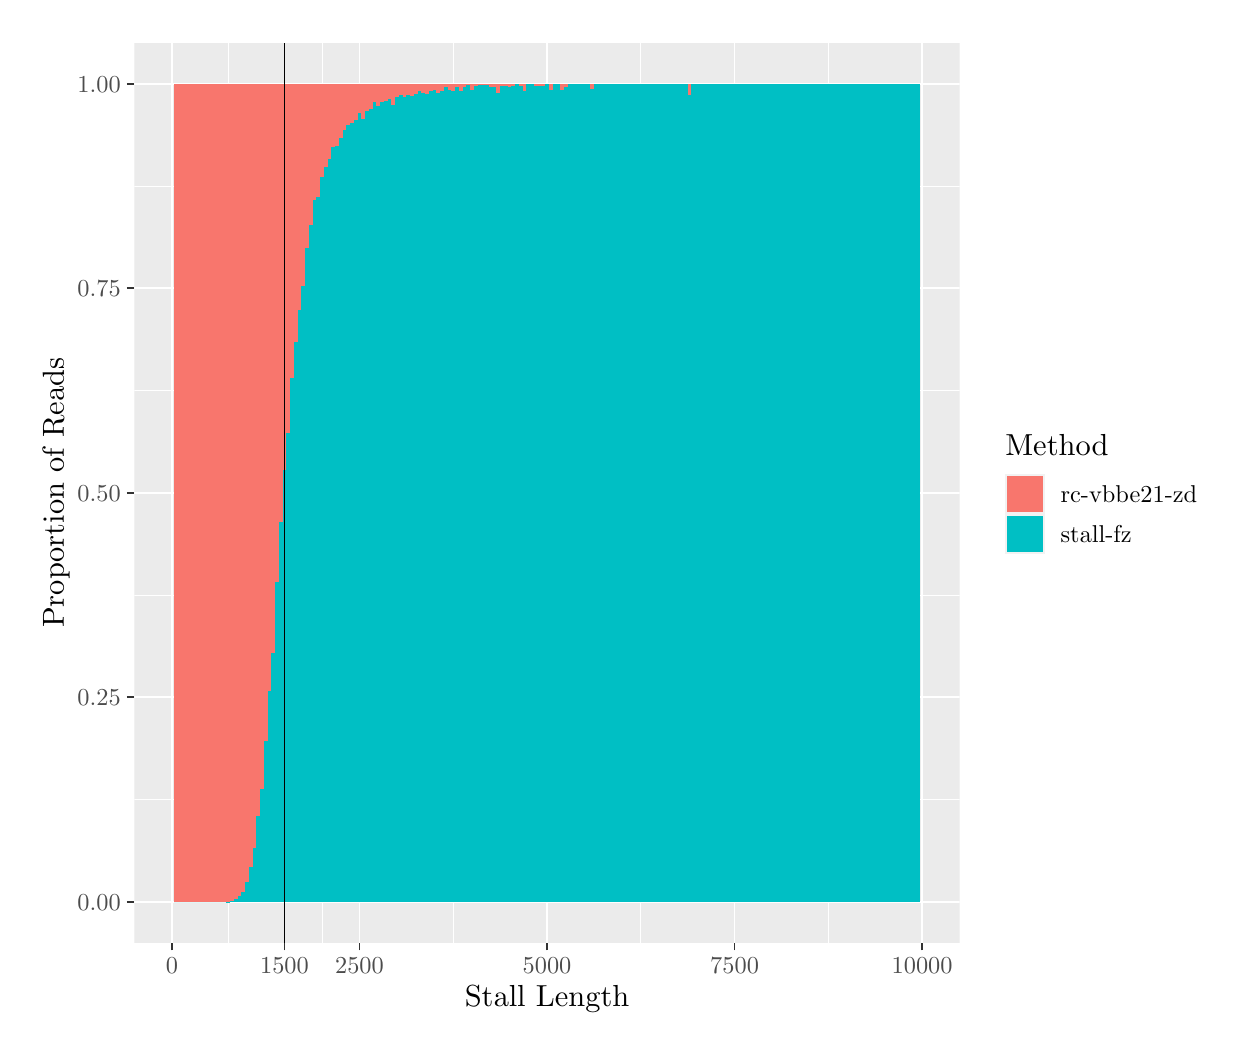
\begin{tikzpicture}[x=1pt,y=1pt]
\definecolor{fillColor}{RGB}{255,255,255}
\path[use as bounding box,fill=fillColor,fill opacity=0.00] (0,0) rectangle (433.62,361.35);
\begin{scope}
\path[clip] (  0.00,  0.00) rectangle (433.62,361.35);
\definecolor{drawColor}{RGB}{255,255,255}
\definecolor{fillColor}{RGB}{255,255,255}

\path[draw=drawColor,line width= 0.6pt,line join=round,line cap=round,fill=fillColor] (  0.00,  0.00) rectangle (433.62,361.35);
\end{scope}
\begin{scope}
\path[clip] ( 38.56, 30.69) rectangle (336.78,355.85);
\definecolor{fillColor}{gray}{0.92}

\path[fill=fillColor] ( 38.56, 30.69) rectangle (336.78,355.85);
\definecolor{drawColor}{RGB}{255,255,255}

\path[draw=drawColor,line width= 0.3pt,line join=round] ( 38.56, 82.42) --
	(336.78, 82.42);

\path[draw=drawColor,line width= 0.3pt,line join=round] ( 38.56,156.32) --
	(336.78,156.32);

\path[draw=drawColor,line width= 0.3pt,line join=round] ( 38.56,230.22) --
	(336.78,230.22);

\path[draw=drawColor,line width= 0.3pt,line join=round] ( 38.56,304.12) --
	(336.78,304.12);

\path[draw=drawColor,line width= 0.3pt,line join=round] ( 72.44, 30.69) --
	( 72.44,355.85);

\path[draw=drawColor,line width= 0.3pt,line join=round] (106.33, 30.69) --
	(106.33,355.85);

\path[draw=drawColor,line width= 0.3pt,line join=round] (153.78, 30.69) --
	(153.78,355.85);

\path[draw=drawColor,line width= 0.3pt,line join=round] (221.55, 30.69) --
	(221.55,355.85);

\path[draw=drawColor,line width= 0.3pt,line join=round] (289.33, 30.69) --
	(289.33,355.85);

\path[draw=drawColor,line width= 0.6pt,line join=round] ( 38.56, 45.47) --
	(336.78, 45.47);

\path[draw=drawColor,line width= 0.6pt,line join=round] ( 38.56,119.37) --
	(336.78,119.37);

\path[draw=drawColor,line width= 0.6pt,line join=round] ( 38.56,193.27) --
	(336.78,193.27);

\path[draw=drawColor,line width= 0.6pt,line join=round] ( 38.56,267.17) --
	(336.78,267.17);

\path[draw=drawColor,line width= 0.6pt,line join=round] ( 38.56,341.07) --
	(336.78,341.07);

\path[draw=drawColor,line width= 0.6pt,line join=round] ( 52.11, 30.69) --
	( 52.11,355.85);

\path[draw=drawColor,line width= 0.6pt,line join=round] ( 92.78, 30.69) --
	( 92.78,355.85);

\path[draw=drawColor,line width= 0.6pt,line join=round] (119.89, 30.69) --
	(119.89,355.85);

\path[draw=drawColor,line width= 0.6pt,line join=round] (187.67, 30.69) --
	(187.67,355.85);

\path[draw=drawColor,line width= 0.6pt,line join=round] (255.44, 30.69) --
	(255.44,355.85);

\path[draw=drawColor,line width= 0.6pt,line join=round] (323.22, 30.69) --
	(323.22,355.85);
\definecolor{fillColor}{RGB}{248,118,109}

\path[fill=fillColor] ( 52.79, 45.47) rectangle ( 54.14,341.07);

\path[fill=fillColor] ( 54.14, 45.47) rectangle ( 55.50,341.07);

\path[fill=fillColor] ( 55.50, 45.47) rectangle ( 56.85,341.07);

\path[fill=fillColor] ( 56.85, 45.47) rectangle ( 58.21,341.07);

\path[fill=fillColor] ( 58.21, 45.47) rectangle ( 59.57,341.07);

\path[fill=fillColor] ( 59.57, 45.47) rectangle ( 60.92,341.07);

\path[fill=fillColor] ( 60.92, 45.47) rectangle ( 62.28,341.07);

\path[fill=fillColor] ( 62.28, 45.47) rectangle ( 63.63,341.07);

\path[fill=fillColor] ( 63.63, 45.47) rectangle ( 64.99,341.07);

\path[fill=fillColor] ( 64.99, 45.47) rectangle ( 66.34,341.07);

\path[fill=fillColor] ( 66.34, 45.47) rectangle ( 67.70,341.07);

\path[fill=fillColor] ( 67.70, 45.47) rectangle ( 69.05,341.07);

\path[fill=fillColor] ( 69.05, 45.47) rectangle ( 70.41,341.07);

\path[fill=fillColor] ( 70.41, 45.47) rectangle ( 71.77,341.07);

\path[fill=fillColor] ( 71.77, 45.49) rectangle ( 73.12,341.07);

\path[fill=fillColor] ( 73.12, 45.92) rectangle ( 74.48,341.07);

\path[fill=fillColor] ( 74.48, 46.32) rectangle ( 75.83,341.07);

\path[fill=fillColor] ( 75.83, 47.48) rectangle ( 77.19,341.07);

\path[fill=fillColor] ( 77.19, 48.95) rectangle ( 78.54,341.07);

\path[fill=fillColor] ( 78.54, 52.57) rectangle ( 79.90,341.07);

\path[fill=fillColor] ( 79.90, 57.99) rectangle ( 81.25,341.07);

\path[fill=fillColor] ( 81.25, 64.89) rectangle ( 82.61,341.07);

\path[fill=fillColor] ( 82.61, 76.64) rectangle ( 83.97,341.07);

\path[fill=fillColor] ( 83.97, 86.37) rectangle ( 85.32,341.07);

\path[fill=fillColor] ( 85.32,103.73) rectangle ( 86.68,341.07);

\path[fill=fillColor] ( 86.68,121.80) rectangle ( 88.03,341.07);

\path[fill=fillColor] ( 88.03,135.40) rectangle ( 89.39,341.07);

\path[fill=fillColor] ( 89.39,161.09) rectangle ( 90.74,341.07);

\path[fill=fillColor] ( 90.74,182.61) rectangle ( 92.10,341.07);

\path[fill=fillColor] ( 92.10,201.69) rectangle ( 93.45,341.07);

\path[fill=fillColor] ( 93.45,214.83) rectangle ( 94.81,341.07);

\path[fill=fillColor] ( 94.81,234.71) rectangle ( 96.17,341.07);

\path[fill=fillColor] ( 96.17,247.88) rectangle ( 97.52,341.07);

\path[fill=fillColor] ( 97.52,259.33) rectangle ( 98.88,341.07);

\path[fill=fillColor] ( 98.88,268.04) rectangle (100.23,341.07);

\path[fill=fillColor] (100.23,281.77) rectangle (101.59,341.07);

\path[fill=fillColor] (101.59,290.15) rectangle (102.94,341.07);

\path[fill=fillColor] (102.94,299.08) rectangle (104.30,341.07);

\path[fill=fillColor] (104.30,300.06) rectangle (105.65,341.07);

\path[fill=fillColor] (105.65,307.56) rectangle (107.01,341.07);

\path[fill=fillColor] (107.01,310.83) rectangle (108.37,341.07);

\path[fill=fillColor] (108.37,313.71) rectangle (109.72,341.07);

\path[fill=fillColor] (109.72,318.32) rectangle (111.08,341.07);

\path[fill=fillColor] (111.08,318.61) rectangle (112.43,341.07);

\path[fill=fillColor] (112.43,321.62) rectangle (113.79,341.07);

\path[fill=fillColor] (113.79,324.46) rectangle (115.14,341.07);

\path[fill=fillColor] (115.14,326.00) rectangle (116.50,341.07);

\path[fill=fillColor] (116.50,326.99) rectangle (117.85,341.07);

\path[fill=fillColor] (117.85,328.11) rectangle (119.21,341.07);

\path[fill=fillColor] (119.21,330.49) rectangle (120.57,341.07);

\path[fill=fillColor] (120.57,328.48) rectangle (121.92,341.07);

\path[fill=fillColor] (121.92,331.26) rectangle (123.28,341.07);

\path[fill=fillColor] (123.28,331.80) rectangle (124.63,341.07);

\path[fill=fillColor] (124.63,334.52) rectangle (125.99,341.07);

\path[fill=fillColor] (125.99,333.20) rectangle (127.34,341.07);

\path[fill=fillColor] (127.34,334.33) rectangle (128.70,341.07);

\path[fill=fillColor] (128.70,334.88) rectangle (130.05,341.07);

\path[fill=fillColor] (130.05,335.69) rectangle (131.41,341.07);

\path[fill=fillColor] (131.41,333.30) rectangle (132.77,341.07);

\path[fill=fillColor] (132.77,336.15) rectangle (134.12,341.07);

\path[fill=fillColor] (134.12,336.96) rectangle (135.48,341.07);

\path[fill=fillColor] (135.48,336.47) rectangle (136.83,341.07);

\path[fill=fillColor] (136.83,337.17) rectangle (138.19,341.07);

\path[fill=fillColor] (138.19,336.65) rectangle (139.54,341.07);

\path[fill=fillColor] (139.54,337.46) rectangle (140.90,341.07);

\path[fill=fillColor] (140.90,338.46) rectangle (142.25,341.07);

\path[fill=fillColor] (142.25,337.85) rectangle (143.61,341.07);

\path[fill=fillColor] (143.61,337.32) rectangle (144.97,341.07);

\path[fill=fillColor] (144.97,338.55) rectangle (146.32,341.07);

\path[fill=fillColor] (146.32,338.66) rectangle (147.68,341.07);

\path[fill=fillColor] (147.68,337.90) rectangle (149.03,341.07);

\path[fill=fillColor] (149.03,338.44) rectangle (150.39,341.07);

\path[fill=fillColor] (150.39,339.75) rectangle (151.74,341.07);

\path[fill=fillColor] (151.74,338.93) rectangle (153.10,341.07);

\path[fill=fillColor] (153.10,338.63) rectangle (154.45,341.07);

\path[fill=fillColor] (154.45,339.91) rectangle (155.81,341.07);

\path[fill=fillColor] (155.81,338.52) rectangle (157.17,341.07);

\path[fill=fillColor] (157.17,339.80) rectangle (158.52,341.07);

\path[fill=fillColor] (158.52,340.63) rectangle (159.88,341.07);

\path[fill=fillColor] (159.88,338.85) rectangle (161.23,341.07);

\path[fill=fillColor] (161.23,340.14) rectangle (162.59,341.07);

\path[fill=fillColor] (162.59,340.59) rectangle (163.94,341.07);

\path[fill=fillColor] (163.94,340.58) rectangle (165.30,341.07);

\path[fill=fillColor] (165.30,340.53) rectangle (166.65,341.07);

\path[fill=fillColor] (166.65,339.91) rectangle (168.01,341.07);

\path[fill=fillColor] (168.01,339.95) rectangle (169.37,341.07);

\path[fill=fillColor] (169.37,337.56) rectangle (170.72,341.07);

\path[fill=fillColor] (170.72,340.42) rectangle (172.08,341.07);

\path[fill=fillColor] (172.08,340.40) rectangle (173.43,341.07);

\path[fill=fillColor] (173.43,339.76) rectangle (174.79,341.07);

\path[fill=fillColor] (174.79,340.31) rectangle (176.14,341.07);

\path[fill=fillColor] (176.14,341.07) rectangle (177.50,341.07);

\path[fill=fillColor] (177.50,340.29) rectangle (178.85,341.07);

\path[fill=fillColor] (178.85,338.62) rectangle (180.21,341.07);

\path[fill=fillColor] (180.21,341.07) rectangle (181.57,341.07);

\path[fill=fillColor] (181.57,341.07) rectangle (182.92,341.07);

\path[fill=fillColor] (182.92,340.22) rectangle (184.28,341.07);

\path[fill=fillColor] (184.28,340.23) rectangle (185.63,341.07);

\path[fill=fillColor] (185.63,340.17) rectangle (186.99,341.07);

\path[fill=fillColor] (186.99,341.07) rectangle (188.34,341.07);

\path[fill=fillColor] (188.34,338.90) rectangle (189.70,341.07);

\path[fill=fillColor] (189.70,341.07) rectangle (191.05,341.07);

\path[fill=fillColor] (191.05,341.07) rectangle (192.41,341.07);

\path[fill=fillColor] (192.41,338.74) rectangle (193.77,341.07);

\path[fill=fillColor] (193.77,339.77) rectangle (195.12,341.07);

\path[fill=fillColor] (195.12,341.07) rectangle (196.48,341.07);

\path[fill=fillColor] (196.48,341.07) rectangle (197.83,341.07);

\path[fill=fillColor] (197.83,341.07) rectangle (199.19,341.07);

\path[fill=fillColor] (199.19,341.07) rectangle (200.54,341.07);

\path[fill=fillColor] (200.54,341.07) rectangle (201.90,341.07);

\path[fill=fillColor] (201.90,341.07) rectangle (203.25,341.07);

\path[fill=fillColor] (203.25,339.32) rectangle (204.61,341.07);

\path[fill=fillColor] (204.61,341.07) rectangle (205.97,341.07);

\path[fill=fillColor] (205.97,341.07) rectangle (207.32,341.07);

\path[fill=fillColor] (207.32,341.07) rectangle (208.68,341.07);

\path[fill=fillColor] (208.68,341.07) rectangle (210.03,341.07);

\path[fill=fillColor] (210.03,341.07) rectangle (211.39,341.07);

\path[fill=fillColor] (211.39,341.07) rectangle (212.74,341.07);

\path[fill=fillColor] (212.74,341.07) rectangle (214.10,341.07);

\path[fill=fillColor] (214.10,341.07) rectangle (215.45,341.07);

\path[fill=fillColor] (215.45,341.07) rectangle (216.81,341.07);

\path[fill=fillColor] (216.81,341.07) rectangle (218.17,341.07);

\path[fill=fillColor] (218.17,341.07) rectangle (219.52,341.07);

\path[fill=fillColor] (219.52,341.07) rectangle (220.88,341.07);

\path[fill=fillColor] (220.88,341.07) rectangle (222.23,341.07);

\path[fill=fillColor] (222.23,341.07) rectangle (223.59,341.07);

\path[fill=fillColor] (223.59,341.07) rectangle (224.94,341.07);

\path[fill=fillColor] (224.94,341.07) rectangle (226.30,341.07);

\path[fill=fillColor] (226.30,341.07) rectangle (227.65,341.07);

\path[fill=fillColor] (227.65,341.07) rectangle (229.01,341.07);

\path[fill=fillColor] (229.01,341.07) rectangle (230.37,341.07);

\path[fill=fillColor] (230.37,341.07) rectangle (231.72,341.07);

\path[fill=fillColor] (231.72,341.07) rectangle (233.08,341.07);

\path[fill=fillColor] (233.08,341.07) rectangle (234.43,341.07);

\path[fill=fillColor] (234.43,341.07) rectangle (235.79,341.07);

\path[fill=fillColor] (235.79,341.07) rectangle (237.14,341.07);

\path[fill=fillColor] (237.14,341.07) rectangle (238.50,341.07);

\path[fill=fillColor] (238.50,337.13) rectangle (239.85,341.07);

\path[fill=fillColor] (239.85,341.07) rectangle (241.21,341.07);

\path[fill=fillColor] (241.21,341.07) rectangle (242.56,341.07);

\path[fill=fillColor] (242.56,341.07) rectangle (243.92,341.07);

\path[fill=fillColor] (243.92,341.07) rectangle (245.28,341.07);

\path[fill=fillColor] (245.28,341.07) rectangle (246.63,341.07);

\path[fill=fillColor] (246.63,341.07) rectangle (247.99,341.07);

\path[fill=fillColor] (247.99,341.07) rectangle (249.34,341.07);

\path[fill=fillColor] (249.34,341.07) rectangle (250.70,341.07);

\path[fill=fillColor] (250.70,341.07) rectangle (252.05,341.07);

\path[fill=fillColor] (252.05,341.07) rectangle (253.41,341.07);

\path[fill=fillColor] (253.41,341.07) rectangle (254.76,341.07);

\path[fill=fillColor] (254.76,341.07) rectangle (256.12,341.07);

\path[fill=fillColor] (256.12,341.07) rectangle (257.48,341.07);

\path[fill=fillColor] (257.48,341.07) rectangle (258.83,341.07);

\path[fill=fillColor] (258.83,341.07) rectangle (260.19,341.07);

\path[fill=fillColor] (260.19,341.07) rectangle (261.54,341.07);

\path[fill=fillColor] (261.54,341.07) rectangle (262.90,341.07);

\path[fill=fillColor] (262.90,341.07) rectangle (264.25,341.07);

\path[fill=fillColor] (264.25,341.07) rectangle (265.61,341.07);

\path[fill=fillColor] (265.61,341.07) rectangle (266.96,341.07);

\path[fill=fillColor] (266.96,341.07) rectangle (268.32,341.07);

\path[fill=fillColor] (268.32,341.07) rectangle (269.68,341.07);

\path[fill=fillColor] (269.68,341.07) rectangle (271.03,341.07);

\path[fill=fillColor] (271.03,341.07) rectangle (272.39,341.07);

\path[fill=fillColor] (272.39,341.07) rectangle (273.74,341.07);

\path[fill=fillColor] (273.74,341.07) rectangle (275.10,341.07);

\path[fill=fillColor] (275.10,341.07) rectangle (276.45,341.07);

\path[fill=fillColor] (276.45,341.07) rectangle (277.81,341.07);

\path[fill=fillColor] (277.81,341.07) rectangle (279.16,341.07);

\path[fill=fillColor] (279.16,341.07) rectangle (280.52,341.07);

\path[fill=fillColor] (280.52,341.07) rectangle (281.88,341.07);

\path[fill=fillColor] (281.88,341.07) rectangle (283.23,341.07);

\path[fill=fillColor] (283.23,341.07) rectangle (284.59,341.07);

\path[fill=fillColor] (284.59,341.07) rectangle (285.94,341.07);

\path[fill=fillColor] (285.94,341.07) rectangle (287.30,341.07);

\path[fill=fillColor] (287.30,341.07) rectangle (288.65,341.07);

\path[fill=fillColor] (288.65,341.07) rectangle (290.01,341.07);

\path[fill=fillColor] (290.01,341.07) rectangle (291.36,341.07);

\path[fill=fillColor] (291.36,341.07) rectangle (292.72,341.07);

\path[fill=fillColor] (292.72,341.07) rectangle (294.08,341.07);

\path[fill=fillColor] (294.08,341.07) rectangle (295.43,341.07);

\path[fill=fillColor] (295.43,341.07) rectangle (296.79,341.07);

\path[fill=fillColor] (296.79,341.07) rectangle (298.14,341.07);

\path[fill=fillColor] (298.14,341.07) rectangle (299.50,341.07);

\path[fill=fillColor] (299.50,341.07) rectangle (300.85,341.07);

\path[fill=fillColor] (300.85,341.07) rectangle (302.21,341.07);

\path[fill=fillColor] (302.21,341.07) rectangle (303.56,341.07);

\path[fill=fillColor] (303.56,341.07) rectangle (304.92,341.07);

\path[fill=fillColor] (304.92,341.07) rectangle (306.28,341.07);

\path[fill=fillColor] (306.28,341.07) rectangle (307.63,341.07);

\path[fill=fillColor] (307.63,341.07) rectangle (308.99,341.07);

\path[fill=fillColor] (308.99,341.07) rectangle (310.34,341.07);

\path[fill=fillColor] (310.34,341.07) rectangle (311.70,341.07);

\path[fill=fillColor] (311.70,341.07) rectangle (313.05,341.07);

\path[fill=fillColor] (313.05,341.07) rectangle (314.41,341.07);

\path[fill=fillColor] (314.41,341.07) rectangle (315.76,341.07);

\path[fill=fillColor] (315.76,341.07) rectangle (317.12,341.07);

\path[fill=fillColor] (317.12,341.07) rectangle (318.48,341.07);

\path[fill=fillColor] (318.48,341.07) rectangle (319.83,341.07);

\path[fill=fillColor] (319.83,341.07) rectangle (321.19,341.07);

\path[fill=fillColor] (321.19,341.07) rectangle (322.54,341.07);
\definecolor{fillColor}{RGB}{0,191,196}

\path[fill=fillColor] ( 52.79, 45.47) rectangle ( 54.14, 45.47);

\path[fill=fillColor] ( 54.14, 45.47) rectangle ( 55.50, 45.47);

\path[fill=fillColor] ( 55.50, 45.47) rectangle ( 56.85, 45.47);

\path[fill=fillColor] ( 56.85, 45.47) rectangle ( 58.21, 45.47);

\path[fill=fillColor] ( 58.21, 45.47) rectangle ( 59.57, 45.47);

\path[fill=fillColor] ( 59.57, 45.47) rectangle ( 60.92, 45.47);

\path[fill=fillColor] ( 60.92, 45.47) rectangle ( 62.28, 45.47);

\path[fill=fillColor] ( 62.28, 45.47) rectangle ( 63.63, 45.47);

\path[fill=fillColor] ( 63.63, 45.47) rectangle ( 64.99, 45.47);

\path[fill=fillColor] ( 64.99, 45.47) rectangle ( 66.34, 45.47);

\path[fill=fillColor] ( 66.34, 45.47) rectangle ( 67.70, 45.47);

\path[fill=fillColor] ( 67.70, 45.47) rectangle ( 69.05, 45.47);

\path[fill=fillColor] ( 69.05, 45.47) rectangle ( 70.41, 45.47);

\path[fill=fillColor] ( 70.41, 45.47) rectangle ( 71.77, 45.47);

\path[fill=fillColor] ( 71.77, 45.47) rectangle ( 73.12, 45.49);

\path[fill=fillColor] ( 73.12, 45.47) rectangle ( 74.48, 45.92);

\path[fill=fillColor] ( 74.48, 45.47) rectangle ( 75.83, 46.32);

\path[fill=fillColor] ( 75.83, 45.47) rectangle ( 77.19, 47.48);

\path[fill=fillColor] ( 77.19, 45.47) rectangle ( 78.54, 48.95);

\path[fill=fillColor] ( 78.54, 45.47) rectangle ( 79.90, 52.57);

\path[fill=fillColor] ( 79.90, 45.47) rectangle ( 81.25, 57.99);

\path[fill=fillColor] ( 81.25, 45.47) rectangle ( 82.61, 64.89);

\path[fill=fillColor] ( 82.61, 45.47) rectangle ( 83.97, 76.64);

\path[fill=fillColor] ( 83.97, 45.47) rectangle ( 85.32, 86.37);

\path[fill=fillColor] ( 85.32, 45.47) rectangle ( 86.68,103.73);

\path[fill=fillColor] ( 86.68, 45.47) rectangle ( 88.03,121.80);

\path[fill=fillColor] ( 88.03, 45.47) rectangle ( 89.39,135.40);

\path[fill=fillColor] ( 89.39, 45.47) rectangle ( 90.74,161.09);

\path[fill=fillColor] ( 90.74, 45.47) rectangle ( 92.10,182.61);

\path[fill=fillColor] ( 92.10, 45.47) rectangle ( 93.45,201.69);

\path[fill=fillColor] ( 93.45, 45.47) rectangle ( 94.81,214.83);

\path[fill=fillColor] ( 94.81, 45.47) rectangle ( 96.17,234.71);

\path[fill=fillColor] ( 96.17, 45.47) rectangle ( 97.52,247.88);

\path[fill=fillColor] ( 97.52, 45.47) rectangle ( 98.88,259.33);

\path[fill=fillColor] ( 98.88, 45.47) rectangle (100.23,268.04);

\path[fill=fillColor] (100.23, 45.47) rectangle (101.59,281.77);

\path[fill=fillColor] (101.59, 45.47) rectangle (102.94,290.15);

\path[fill=fillColor] (102.94, 45.47) rectangle (104.30,299.08);

\path[fill=fillColor] (104.30, 45.47) rectangle (105.65,300.06);

\path[fill=fillColor] (105.65, 45.47) rectangle (107.01,307.56);

\path[fill=fillColor] (107.01, 45.47) rectangle (108.37,310.83);

\path[fill=fillColor] (108.37, 45.47) rectangle (109.72,313.71);

\path[fill=fillColor] (109.72, 45.47) rectangle (111.08,318.32);

\path[fill=fillColor] (111.08, 45.47) rectangle (112.43,318.61);

\path[fill=fillColor] (112.43, 45.47) rectangle (113.79,321.62);

\path[fill=fillColor] (113.79, 45.47) rectangle (115.14,324.46);

\path[fill=fillColor] (115.14, 45.47) rectangle (116.50,326.00);

\path[fill=fillColor] (116.50, 45.47) rectangle (117.85,326.99);

\path[fill=fillColor] (117.85, 45.47) rectangle (119.21,328.11);

\path[fill=fillColor] (119.21, 45.47) rectangle (120.57,330.49);

\path[fill=fillColor] (120.57, 45.47) rectangle (121.92,328.48);

\path[fill=fillColor] (121.92, 45.47) rectangle (123.28,331.26);

\path[fill=fillColor] (123.28, 45.47) rectangle (124.63,331.80);

\path[fill=fillColor] (124.63, 45.47) rectangle (125.99,334.52);

\path[fill=fillColor] (125.99, 45.47) rectangle (127.34,333.20);

\path[fill=fillColor] (127.34, 45.47) rectangle (128.70,334.33);

\path[fill=fillColor] (128.70, 45.47) rectangle (130.05,334.88);

\path[fill=fillColor] (130.05, 45.47) rectangle (131.41,335.69);

\path[fill=fillColor] (131.41, 45.47) rectangle (132.77,333.30);

\path[fill=fillColor] (132.77, 45.47) rectangle (134.12,336.15);

\path[fill=fillColor] (134.12, 45.47) rectangle (135.48,336.96);

\path[fill=fillColor] (135.48, 45.47) rectangle (136.83,336.47);

\path[fill=fillColor] (136.83, 45.47) rectangle (138.19,337.17);

\path[fill=fillColor] (138.19, 45.47) rectangle (139.54,336.65);

\path[fill=fillColor] (139.54, 45.47) rectangle (140.90,337.46);

\path[fill=fillColor] (140.90, 45.47) rectangle (142.25,338.46);

\path[fill=fillColor] (142.25, 45.47) rectangle (143.61,337.85);

\path[fill=fillColor] (143.61, 45.47) rectangle (144.97,337.32);

\path[fill=fillColor] (144.97, 45.47) rectangle (146.32,338.55);

\path[fill=fillColor] (146.32, 45.47) rectangle (147.68,338.66);

\path[fill=fillColor] (147.68, 45.47) rectangle (149.03,337.90);

\path[fill=fillColor] (149.03, 45.47) rectangle (150.39,338.44);

\path[fill=fillColor] (150.39, 45.47) rectangle (151.74,339.75);

\path[fill=fillColor] (151.74, 45.47) rectangle (153.10,338.93);

\path[fill=fillColor] (153.10, 45.47) rectangle (154.45,338.63);

\path[fill=fillColor] (154.45, 45.47) rectangle (155.81,339.91);

\path[fill=fillColor] (155.81, 45.47) rectangle (157.17,338.52);

\path[fill=fillColor] (157.17, 45.47) rectangle (158.52,339.80);

\path[fill=fillColor] (158.52, 45.47) rectangle (159.88,340.63);

\path[fill=fillColor] (159.88, 45.47) rectangle (161.23,338.85);

\path[fill=fillColor] (161.23, 45.47) rectangle (162.59,340.14);

\path[fill=fillColor] (162.59, 45.47) rectangle (163.94,340.59);

\path[fill=fillColor] (163.94, 45.47) rectangle (165.30,340.58);

\path[fill=fillColor] (165.30, 45.47) rectangle (166.65,340.53);

\path[fill=fillColor] (166.65, 45.47) rectangle (168.01,339.91);

\path[fill=fillColor] (168.01, 45.47) rectangle (169.37,339.95);

\path[fill=fillColor] (169.37, 45.47) rectangle (170.72,337.56);

\path[fill=fillColor] (170.72, 45.47) rectangle (172.08,340.42);

\path[fill=fillColor] (172.08, 45.47) rectangle (173.43,340.40);

\path[fill=fillColor] (173.43, 45.47) rectangle (174.79,339.76);

\path[fill=fillColor] (174.79, 45.47) rectangle (176.14,340.31);

\path[fill=fillColor] (176.14, 45.47) rectangle (177.50,341.07);

\path[fill=fillColor] (177.50, 45.47) rectangle (178.85,340.29);

\path[fill=fillColor] (178.85, 45.47) rectangle (180.21,338.62);

\path[fill=fillColor] (180.21, 45.47) rectangle (181.57,341.07);

\path[fill=fillColor] (181.57, 45.47) rectangle (182.92,341.07);

\path[fill=fillColor] (182.92, 45.47) rectangle (184.28,340.22);

\path[fill=fillColor] (184.28, 45.47) rectangle (185.63,340.23);

\path[fill=fillColor] (185.63, 45.47) rectangle (186.99,340.17);

\path[fill=fillColor] (186.99, 45.47) rectangle (188.34,341.07);

\path[fill=fillColor] (188.34, 45.47) rectangle (189.70,338.90);

\path[fill=fillColor] (189.70, 45.47) rectangle (191.05,341.07);

\path[fill=fillColor] (191.05, 45.47) rectangle (192.41,341.07);

\path[fill=fillColor] (192.41, 45.47) rectangle (193.77,338.74);

\path[fill=fillColor] (193.77, 45.47) rectangle (195.12,339.77);

\path[fill=fillColor] (195.12, 45.47) rectangle (196.48,341.07);

\path[fill=fillColor] (196.48, 45.47) rectangle (197.83,341.07);

\path[fill=fillColor] (197.83, 45.47) rectangle (199.19,341.07);

\path[fill=fillColor] (199.19, 45.47) rectangle (200.54,341.07);

\path[fill=fillColor] (200.54, 45.47) rectangle (201.90,341.07);

\path[fill=fillColor] (201.90, 45.47) rectangle (203.25,341.07);

\path[fill=fillColor] (203.25, 45.47) rectangle (204.61,339.32);

\path[fill=fillColor] (204.61, 45.47) rectangle (205.97,341.07);

\path[fill=fillColor] (205.97, 45.47) rectangle (207.32,341.07);

\path[fill=fillColor] (207.32, 45.47) rectangle (208.68,341.07);

\path[fill=fillColor] (208.68, 45.47) rectangle (210.03,341.07);

\path[fill=fillColor] (210.03, 45.47) rectangle (211.39,341.07);

\path[fill=fillColor] (211.39, 45.47) rectangle (212.74,341.07);

\path[fill=fillColor] (212.74, 45.47) rectangle (214.10,341.07);

\path[fill=fillColor] (214.10, 45.47) rectangle (215.45,341.07);

\path[fill=fillColor] (215.45, 45.47) rectangle (216.81,341.07);

\path[fill=fillColor] (216.81, 45.47) rectangle (218.17,341.07);

\path[fill=fillColor] (218.17, 45.47) rectangle (219.52,341.07);

\path[fill=fillColor] (219.52, 45.47) rectangle (220.88,341.07);

\path[fill=fillColor] (220.88, 45.47) rectangle (222.23,341.07);

\path[fill=fillColor] (222.23, 45.47) rectangle (223.59,341.07);

\path[fill=fillColor] (223.59, 45.47) rectangle (224.94,341.07);

\path[fill=fillColor] (224.94, 45.47) rectangle (226.30,341.07);

\path[fill=fillColor] (226.30, 45.47) rectangle (227.65,341.07);

\path[fill=fillColor] (227.65, 45.47) rectangle (229.01,341.07);

\path[fill=fillColor] (229.01, 45.47) rectangle (230.37,341.07);

\path[fill=fillColor] (230.37, 45.47) rectangle (231.72,341.07);

\path[fill=fillColor] (231.72, 45.47) rectangle (233.08,341.07);

\path[fill=fillColor] (233.08, 45.47) rectangle (234.43,341.07);

\path[fill=fillColor] (234.43, 45.47) rectangle (235.79,341.07);

\path[fill=fillColor] (235.79, 45.47) rectangle (237.14,341.07);

\path[fill=fillColor] (237.14, 45.47) rectangle (238.50,341.07);

\path[fill=fillColor] (238.50, 45.47) rectangle (239.85,337.13);

\path[fill=fillColor] (239.85, 45.47) rectangle (241.21,341.07);

\path[fill=fillColor] (241.21, 45.47) rectangle (242.56,341.07);

\path[fill=fillColor] (242.56, 45.47) rectangle (243.92,341.07);

\path[fill=fillColor] (243.92, 45.47) rectangle (245.28,341.07);

\path[fill=fillColor] (245.28, 45.47) rectangle (246.63,341.07);

\path[fill=fillColor] (246.63, 45.47) rectangle (247.99,341.07);

\path[fill=fillColor] (247.99, 45.47) rectangle (249.34,341.07);

\path[fill=fillColor] (249.34, 45.47) rectangle (250.70,341.07);

\path[fill=fillColor] (250.70, 45.47) rectangle (252.05,341.07);

\path[fill=fillColor] (252.05, 45.47) rectangle (253.41,341.07);

\path[fill=fillColor] (253.41, 45.47) rectangle (254.76,341.07);

\path[fill=fillColor] (254.76, 45.47) rectangle (256.12,341.07);

\path[fill=fillColor] (256.12, 45.47) rectangle (257.48,341.07);

\path[fill=fillColor] (257.48, 45.47) rectangle (258.83,341.07);

\path[fill=fillColor] (258.83, 45.47) rectangle (260.19,341.07);

\path[fill=fillColor] (260.19, 45.47) rectangle (261.54,341.07);

\path[fill=fillColor] (261.54, 45.47) rectangle (262.90,341.07);

\path[fill=fillColor] (262.90, 45.47) rectangle (264.25,341.07);

\path[fill=fillColor] (264.25, 45.47) rectangle (265.61,341.07);

\path[fill=fillColor] (265.61, 45.47) rectangle (266.96,341.07);

\path[fill=fillColor] (266.96, 45.47) rectangle (268.32,341.07);

\path[fill=fillColor] (268.32, 45.47) rectangle (269.68,341.07);

\path[fill=fillColor] (269.68, 45.47) rectangle (271.03,341.07);

\path[fill=fillColor] (271.03, 45.47) rectangle (272.39,341.07);

\path[fill=fillColor] (272.39, 45.47) rectangle (273.74,341.07);

\path[fill=fillColor] (273.74, 45.47) rectangle (275.10,341.07);

\path[fill=fillColor] (275.10, 45.47) rectangle (276.45,341.07);

\path[fill=fillColor] (276.45, 45.47) rectangle (277.81,341.07);

\path[fill=fillColor] (277.81, 45.47) rectangle (279.16,341.07);

\path[fill=fillColor] (279.16, 45.47) rectangle (280.52,341.07);

\path[fill=fillColor] (280.52, 45.47) rectangle (281.88,341.07);

\path[fill=fillColor] (281.88, 45.47) rectangle (283.23,341.07);

\path[fill=fillColor] (283.23, 45.47) rectangle (284.59,341.07);

\path[fill=fillColor] (284.59, 45.47) rectangle (285.94,341.07);

\path[fill=fillColor] (285.94, 45.47) rectangle (287.30,341.07);

\path[fill=fillColor] (287.30, 45.47) rectangle (288.65,341.07);

\path[fill=fillColor] (288.65, 45.47) rectangle (290.01,341.07);

\path[fill=fillColor] (290.01, 45.47) rectangle (291.36,341.07);

\path[fill=fillColor] (291.36, 45.47) rectangle (292.72,341.07);

\path[fill=fillColor] (292.72, 45.47) rectangle (294.08,341.07);

\path[fill=fillColor] (294.08, 45.47) rectangle (295.43,341.07);

\path[fill=fillColor] (295.43, 45.47) rectangle (296.79,341.07);

\path[fill=fillColor] (296.79, 45.47) rectangle (298.14,341.07);

\path[fill=fillColor] (298.14, 45.47) rectangle (299.50,341.07);

\path[fill=fillColor] (299.50, 45.47) rectangle (300.85,341.07);

\path[fill=fillColor] (300.85, 45.47) rectangle (302.21,341.07);

\path[fill=fillColor] (302.21, 45.47) rectangle (303.56,341.07);

\path[fill=fillColor] (303.56, 45.47) rectangle (304.92,341.07);

\path[fill=fillColor] (304.92, 45.47) rectangle (306.28,341.07);

\path[fill=fillColor] (306.28, 45.47) rectangle (307.63,341.07);

\path[fill=fillColor] (307.63, 45.47) rectangle (308.99,341.07);

\path[fill=fillColor] (308.99, 45.47) rectangle (310.34,341.07);

\path[fill=fillColor] (310.34, 45.47) rectangle (311.70,341.07);

\path[fill=fillColor] (311.70, 45.47) rectangle (313.05,341.07);

\path[fill=fillColor] (313.05, 45.47) rectangle (314.41,341.07);

\path[fill=fillColor] (314.41, 45.47) rectangle (315.76,341.07);

\path[fill=fillColor] (315.76, 45.47) rectangle (317.12,341.07);

\path[fill=fillColor] (317.12, 45.47) rectangle (318.48,341.07);

\path[fill=fillColor] (318.48, 45.47) rectangle (319.83,341.07);

\path[fill=fillColor] (319.83, 45.47) rectangle (321.19,341.07);

\path[fill=fillColor] (321.19, 45.47) rectangle (322.54,341.07);
\definecolor{drawColor}{RGB}{0,0,0}

\path[draw=drawColor,line width= 0.6pt,line join=round] ( 92.78, 30.69) -- ( 92.78,355.85);
\end{scope}
\begin{scope}
\path[clip] (  0.00,  0.00) rectangle (433.62,361.35);
\definecolor{drawColor}{gray}{0.30}

\node[text=drawColor,anchor=base east,inner sep=0pt, outer sep=0pt, scale=  0.88] at ( 33.61, 42.44) {0.00};

\node[text=drawColor,anchor=base east,inner sep=0pt, outer sep=0pt, scale=  0.88] at ( 33.61,116.34) {0.25};

\node[text=drawColor,anchor=base east,inner sep=0pt, outer sep=0pt, scale=  0.88] at ( 33.61,190.24) {0.50};

\node[text=drawColor,anchor=base east,inner sep=0pt, outer sep=0pt, scale=  0.88] at ( 33.61,264.14) {0.75};

\node[text=drawColor,anchor=base east,inner sep=0pt, outer sep=0pt, scale=  0.88] at ( 33.61,338.04) {1.00};
\end{scope}
\begin{scope}
\path[clip] (  0.00,  0.00) rectangle (433.62,361.35);
\definecolor{drawColor}{gray}{0.20}

\path[draw=drawColor,line width= 0.6pt,line join=round] ( 35.81, 45.47) --
	( 38.56, 45.47);

\path[draw=drawColor,line width= 0.6pt,line join=round] ( 35.81,119.37) --
	( 38.56,119.37);

\path[draw=drawColor,line width= 0.6pt,line join=round] ( 35.81,193.27) --
	( 38.56,193.27);

\path[draw=drawColor,line width= 0.6pt,line join=round] ( 35.81,267.17) --
	( 38.56,267.17);

\path[draw=drawColor,line width= 0.6pt,line join=round] ( 35.81,341.07) --
	( 38.56,341.07);
\end{scope}
\begin{scope}
\path[clip] (  0.00,  0.00) rectangle (433.62,361.35);
\definecolor{drawColor}{gray}{0.20}

\path[draw=drawColor,line width= 0.6pt,line join=round] ( 52.11, 27.94) --
	( 52.11, 30.69);

\path[draw=drawColor,line width= 0.6pt,line join=round] ( 92.78, 27.94) --
	( 92.78, 30.69);

\path[draw=drawColor,line width= 0.6pt,line join=round] (119.89, 27.94) --
	(119.89, 30.69);

\path[draw=drawColor,line width= 0.6pt,line join=round] (187.67, 27.94) --
	(187.67, 30.69);

\path[draw=drawColor,line width= 0.6pt,line join=round] (255.44, 27.94) --
	(255.44, 30.69);

\path[draw=drawColor,line width= 0.6pt,line join=round] (323.22, 27.94) --
	(323.22, 30.69);
\end{scope}
\begin{scope}
\path[clip] (  0.00,  0.00) rectangle (433.62,361.35);
\definecolor{drawColor}{gray}{0.30}

\node[text=drawColor,anchor=base,inner sep=0pt, outer sep=0pt, scale=  0.88] at ( 52.11, 19.68) {0};

\node[text=drawColor,anchor=base,inner sep=0pt, outer sep=0pt, scale=  0.88] at ( 92.78, 19.68) {1500};

\node[text=drawColor,anchor=base,inner sep=0pt, outer sep=0pt, scale=  0.88] at (119.89, 19.68) {2500};

\node[text=drawColor,anchor=base,inner sep=0pt, outer sep=0pt, scale=  0.88] at (187.67, 19.68) {5000};

\node[text=drawColor,anchor=base,inner sep=0pt, outer sep=0pt, scale=  0.88] at (255.44, 19.68) {7500};

\node[text=drawColor,anchor=base,inner sep=0pt, outer sep=0pt, scale=  0.88] at (323.22, 19.68) {10000};
\end{scope}
\begin{scope}
\path[clip] (  0.00,  0.00) rectangle (433.62,361.35);
\definecolor{drawColor}{RGB}{0,0,0}

\node[text=drawColor,anchor=base,inner sep=0pt, outer sep=0pt, scale=  1.10] at (187.67,  7.64) {Stall Length};
\end{scope}
\begin{scope}
\path[clip] (  0.00,  0.00) rectangle (433.62,361.35);
\definecolor{drawColor}{RGB}{0,0,0}

\node[text=drawColor,rotate= 90.00,anchor=base,inner sep=0pt, outer sep=0pt, scale=  1.10] at ( 13.08,193.27) {Proportion of Reads};
\end{scope}
\begin{scope}
\path[clip] (  0.00,  0.00) rectangle (433.62,361.35);
\definecolor{fillColor}{RGB}{255,255,255}

\path[fill=fillColor] (347.78,165.71) rectangle (428.12,220.83);
\end{scope}
\begin{scope}
\path[clip] (  0.00,  0.00) rectangle (433.62,361.35);
\definecolor{drawColor}{RGB}{0,0,0}

\node[text=drawColor,anchor=base west,inner sep=0pt, outer sep=0pt, scale=  1.10] at (353.28,206.68) {Method};
\end{scope}
\begin{scope}
\path[clip] (  0.00,  0.00) rectangle (433.62,361.35);
\definecolor{fillColor}{gray}{0.95}

\path[fill=fillColor] (353.28,185.66) rectangle (367.73,200.11);
\end{scope}
\begin{scope}
\path[clip] (  0.00,  0.00) rectangle (433.62,361.35);
\definecolor{fillColor}{RGB}{248,118,109}

\path[fill=fillColor] (353.99,186.37) rectangle (367.02,199.40);
\end{scope}
\begin{scope}
\path[clip] (  0.00,  0.00) rectangle (433.62,361.35);
\definecolor{fillColor}{gray}{0.95}

\path[fill=fillColor] (353.28,171.21) rectangle (367.73,185.66);
\end{scope}
\begin{scope}
\path[clip] (  0.00,  0.00) rectangle (433.62,361.35);
\definecolor{fillColor}{RGB}{0,191,196}

\path[fill=fillColor] (353.99,171.92) rectangle (367.02,184.95);
\end{scope}
\begin{scope}
\path[clip] (  0.00,  0.00) rectangle (433.62,361.35);
\definecolor{drawColor}{RGB}{0,0,0}

\node[text=drawColor,anchor=base west,inner sep=0pt, outer sep=0pt, scale=  0.88] at (373.23,189.86) {rc-vbbe21-zd};
\end{scope}
\begin{scope}
\path[clip] (  0.00,  0.00) rectangle (433.62,361.35);
\definecolor{drawColor}{RGB}{0,0,0}

\node[text=drawColor,anchor=base west,inner sep=0pt, outer sep=0pt, scale=  0.88] at (373.23,175.40) {stall-fz};
\end{scope}
\end{tikzpicture}

\caption{\label{fig:stall-ratio}The 100\% stacked histogram of the compression
	methods with the highest compression ratio for all the reads in the data
	versus their stall length. Reads with a stall length $\sim$1500 and
	greater are more likely to be compressed smaller using stall-fz than
	rc-vbbe21-zd.}
\end{figure}

\begin{figure}
\centering
%\input{plots/reads.blow5.test.svbbe21.read.best}
\includegraphics[scale=0.7]{plots/reads.blow5.test.svbbe21.read.update.best.pdf}
	\caption[A scatter plot of the compression methods with
the highest compression ratio on each read out of rc01s-vbbe21-zd and stall-fz.]{\label{fig:stall-best}A scatter plot of the compression methods with
the highest compression ratio on each read out of rc01s-vbbe21-zd and stall-fz. The
best compression ratio is plotted against the length of the read's stall. Reads
with a stall length $\sim$1500 and greater are more likely to be compressed
smaller with stall-fz rather than rc01s-vbbe21-zd.}
\end{figure}

